% !TeX spellcheck = en_GB
%!TEX TS-program = xelatex
%!BIB TS-program = biber
\chapter{Modelling Natural Fibres Using Auxiliary Maps} \label{chap:p7}
\section*{Statement of Contribution}
	This chapter includes a co-authored journal paper. The bibliographic details of the under review paper are:
\begin{itemize}
	\item Javanbakht, Z, Hall, W \& Öchsner, A (2019). “An Element-wise Scheme to Analyse Local Mechanical Anisotropy in Fibre-reinforced Composites”, Material Science and Technology, accepted.
\end{itemize}
	My contribution as the corresponding author to the paper involved: undertaking literature review, classifying the necessary theoretical backgrounds and models, developing the programming code, analysing and discussing the finite element results, drawing figures, preparing tables, writing and editing the manuscript according to my supervisors’ comments.

\Zia\\
\Wayne\\
\vfill
\newpage
% --------------------------------------------------------------------------------------------------

\paragraph{Title} An Element-wise Scheme to Analyse Local Mechanical Anisotropy in Fibre-reinforced Composites
    
 
    
\paragraph{Abstract} Herein, the general constitutive equation of bi-phasic materials equipped with orientation tensor is presented in direct notation. The formulation is refined by some correction factors specific to natural fibre-reinforced composites; then, a planar case is derived. The necessity of local information is emphasised through the introduction of auxiliary maps, which included volume fraction and orientation data. A semi-analytical homogenisation method is introduced through finite element analysis. Auxiliary maps are shown to be a better alternative to the overall orientation of fibres. Global calculations are insensitive to local variations whilst appropriate auxiliary maps offer refined results. Considering the multi-disciplinary application of orientation tensors, the proposed scheme can be used in all areas where local information cannot be disregarded.


\paragraph{Keywords} Orientation tensor; transverse isotropy; natural fibre composite; computational mechanics.

\section{Introduction}
	
	\paragraph{Statistical distribution of orientation} Statistical measurement of orientation in space results in spherical data~\autocite{Fisher.1987}. The `direction' and `orientation' terms are distinguished from each other since a vector designates the former whereas a line or axis is adequate for the latter. Therefore, a unit-length vector ($\tena{d}$) contains the information for both direction and orientation. The loci of the head of all such vectors is a unit 2-sphere, i.e., $\mathbb{S}^2 = \left\{\tena{d} : \lVert \tena{d}\rVert = 1 \right\}$, where $\lVert\op\rVert$ denotes the Frobenius norm. The notion of direction in 3D requires the whole sphere whereas orientation is expressed via the hemisphere, i.e., it suffices for illustration of centro-symmetric statistical distributions. The orientation probability density function (ODF) $\Psi(\tena{d})$ provides the probability of finding a fibre in the direction $\tena{d}$. In 2D, similar arguments hold for a unit 1-sphere (unit circle).
	 
	% Why use fabric tensors?
	Although such distributions can be captured by ODFs, tensors are used as more compact alternatives. They are approximations that mathematically provide more flexibility. For instance, their invariants can be used to develop constitutive laws while objectivity (material frame indifference) is preserved. Moreover, other properties such as the clustering index~\autocite{Ranganathan.1990} can be determined from orientation tensors that might be used to detect inter-region deviation of fibre orientation. Although this statistical index might show more sensitivity in detecting local fibre distribution (in comparison to the eigenvalues of the orientation tensor), it lacks the flexibility provided by a tensorial measure~\autocite{Javanbakht.2019}.

	\paragraph{Terminology} `Orientation tensors', `fabric tensors', `moment tensors' or `structure tensors' are different terms used to indicate quantities that capture the directional dependency of a microstructure. Although all these terms refer to the same mathematical quantity, the use in the literature has been more context-based. Often, orientation tensors are used to acquire the orientation of short fibres in injection moulding~\autocite{Advani.1987} or generally fibre-reinforced composites~\autocite{Muller.2016b}; fabric tensors are used to characterise the direction of granular materials~\autocite{Millet.2007} or porous materials such as snow~\autocite{Srivastava.2010} and bone~\autocite{Odgaard.1997} or quantify the distribution of damage~\autocite{Krajcinovic.2000}; and structure tensors are used for fibrous biological tissue such as cartilage~\autocite{Tomic.2014}. Herein, the term `orientation tensor' will be used as it attempts to quantify the orientation of the meso-structure that could contain any of the aforementioned heterogeneities. In the literature, it is mostly used to point to either the first or third kinds of Cowin's fabric tensors.
	
	% What are the kinds?
	\paragraph{Kinds of orientation tensors} Kanatani~\autocite{Kanatani.1984} introduced the idea of approximating any distribution (more specifically ODFs) using spherical harmonics~\autocite{Jones.1985} as bases for expansion in 3D; three kinds of orientation tensors were introduced to approximate an ODF:
	\begin{enumerate}
		\item The fabric tensor of first kind of order $k$ (moment tensor) is the average of tensor products of directions, see Eq.~\eqref{eq:ot1}. Herein, this kind is called the `averaged orientation tensor' and it is the building block of other types.
		\item The fabric tensors of second kind of order $k$ are the coefficient tensors contracted with the direction vectors as basis of the expansion. They are calculated from the first kind but the coefficients of higher order depend on the lower order ones, which results in an inflexible approximation~\autocite{Kanatani.1984}.
%		
%		is an approximation to an ODF by a single $k$-order tensor.  a polynomial in terms of orientation tensors of the first kind up to order $k$ contracted with tensorial coefficients:
%		\begin{equation}
%			F(\tena{d})\equidef \frac{1}{4\pi}
%			\left(
%			\tenn{C}{2}\dscp\tena{d}^\tenpow{2}+\tenn{C}{4}\dscp\dscp\tena{d}^\tenpow{4}
%			+\tenn{C}{6}\dscp\dscp\dscp\tena{d}^\tenpow{6}
%	 +\ldots
%			\right),
%		\end{equation}
%		where unique obtaining of the coefficients is an ill-posed problem.
		\item The fabric tensor of third kind of order $k$ is calculated from its first kind counterpart by a subtraction; it is equivalent to the traceless symmetric component in the irreducible decomposition of the fabric tensor of first kind.
%	\begin{equation}
%	\tenb{N}^{(2)}\equidef \tenb{N}^\sym - \frac{1}{3}\tr{\tenb{N}}.
%	\end{equation}	
	\end{enumerate}	
		
	% What is fabric tensors? Cowin probably did not coined the term! Kanatani uesd it earlier.
	The term `fabric tensor' was used by Cowin as the second best measure of meso-structure for a porous material after porosity~\autocite{Cowin.1985}. He generalised the previously-discussed idea of fabric ellipsoid~\autocite{Oda.1980} to fabric tensors, i.e., all second-order positive-definite symmetrical tensors characterising `local architectural anisotropy' or `fabric'. Cowin's fundamental assumption was that the direction-dependency of mechanical response follows that of the fabric. Namely, anisotropy could be incorporated into an isotropic elastic tensor via the fabric tensor~\autocite{Shertzer.2011}. Based on this idea, the orientation tensor has been used to create anisotropic models from the isotropic ones, see the alternative model in~\autocite{Zysset.1995}. Cowin also developed tensorial polynomial failure criteria based on the fabric tensors of first kind~\autocite{Cowin.1986}. 

%	\paragraph{Spectral analysis of orientation tensor} Cowin's idea of orientation tensors  describing the orientation of the material manifests itself in spectral analysis, i.e., principal directions of orientation tensor is the same as those of the material. In principal direction, a general tensor becomes diagonal, or equivalently off-diagonal components vanish. In 3D, the second order orientation tensor can have a maximum of three distinct eigenvalues that correspond to three distinct normalised eigenvectors. Namely, three principal directions exist and the symmetry group is all the proper orthogonal rotation tensors. Such material is orthotropic. If two repeated eigenvalues exist, the eigenvectors are on a plane, i.e., any eigenvectors on this plane represents a principal direction. The symmetry group is the all proper orthogonal rotation tensors about the non-repeating eigenvector. Such a material contains an `isotropic plane' and is transversely isotropic. The case of three repeating eigenvectors indicate that every plane is an isotropy plane and the material is called isotropic. This case occurs when the average orientation tensor becomes isotropic, i.e., its deviatoric component is nullified. In conclusion, a second-order orientation tensor with three, two, and one distinct eigenvalues denotes orthotropy, transverse-isotropy, and isotropy, respectively. Identifying other types of symmetry require higher order tensors~\autocite{Shertzer.2011}. For instance, second-order orientation tensors cannot identify a cubic symmetry and just simply reduces to isotropy~\autocite{Cowin.1985}.

	\paragraph{Spectral analysis of orientation tensor} Cowin's idea of using orientation tensors to describe material anisotropy manifests itself in spectral analysis, i.e., principal directions of orientation tensor coincides with those of the material. The most-commonly used second-order orientation tensor with three, two, and one distinct eigenvalues denotes orthotropy, transverse-isotropy, and isotropy, respectively. Identifying lower orders of symmetry require higher order tensors. For instance, second-order orientation tensors cannot identify a cubic symmetry and just simply reduces to isotropy~\autocite{Cowin.1985}. Nevertheless, spectral analysis of the 2nd-order orientation tensor is sufficient for estimating the principal direction of the material~\autocite{Javanbakht.2017c}. 

	\paragraph{Auxiliary Maps} Measures like the orientation tensor, which could provide meso-structural material properties, refine one's understanding about material behaviour; they are called `auxiliary maps (fields)' herein. In the context of fibre-reinforced composites (FRCs), volume fraction and orientation of fibres are omnipresent in the literature---but very often discussed in a global sense. Thus, they might be suggested as the first two auxiliary maps for FRCs. Although the availability of local data as auxiliary maps might be limited, there are few numerical methods in the literature that take advantage of them anyway.  
	
	\paragraph{Embedded elements} Discrete numerical simulation of meso-structure is possible but computationally limited. For example in FRCs, modelling fibres as discrete elements implicitly incorporates auxiliary maps into the finite element model but it is computationally expensive. To reduce the cost, often smaller samples of the material are analysed, e.g., in the form of representative volume elements (RVEs)~\autocite{Javanbakht.2016b,Javanbakht.2016}, which might lead to apparent mechanical properties rather than the true effective ones. Such artefacts can be related to the wall effect of boundary conditions and the sample size that link the obtained properties more to the structure of the realisations rather than those of the ensemble (material)~\autocite{Bohm.2020}.
	
	\paragraph{Multi-phase elements} `Multi-phase element' methods extract integration point properties from auxiliary maps without using any embedded elements. However, they often require additional number of integration points to properly assign the properties from the meso-structure to elements~\autocite{Zohdi.2001}. An additional obstacle is incorporating the anisotropy of the microstructure, which requires an ODF or its discretised version in the form of orientation tensors; the latter is often calculated in finite regions, e.g., layers of soft tissue~\autocite{Gasser.2006} or arbitrary layers in injection moulding~\autocite{Muller.2016}. However, depending on the manufacturing process, e.g., in sheet moulding compound, the orientation of fibres along thickness becomes insignificant while in-plane dispersed or aggregated texture is created for discontinuous fibres~\autocite{Eduljee.2006}. Or in injection moulding, the orientation of the core layer is more planar than the two boundary layers~\autocite{Advani.1987}. Lack of out-of-plane orientation distribution is quantitatively backed up due to vanishing the minimum eigenvalue along thickness, see the provided results in~\autocite{Muller.2016} for a layer-wise approach. 
	
	\paragraph{Natural fibre composites} Although analytical homogenisation schemes might provide a solid base for calculating effective parameters, localisation calculations can be detrimental, e.g., in strength calculation of brittle inclusions~\autocite{Bohm.2020}. Most of the analytical formulations are implemented numerically in a global fashion, i.e., the orientation tensor is used to obtain the overall direction-dependency rather than a local one~\autocite{Spencer.1984}. For the case of natural fibre-reinforced composites (NFRCs), inherent variation of material and geometrical properties, e.g., length-dependent strength~\autocite{Virk.2013}, length-wise non-uniformity~\autocite{Virk.2009}, irregular cross-section~\autocite{Virk.2009}, and sensitivity to hygroscopic effects~\autocite{Javanbakht.2017b}, adds to the complications of the analysis. Such statistical variations also motivate for a closer look at the homogenisation process in order to obtain a more refined smeared response.	


	
	% TODO add my own paper as in preparation...



	
	
	\paragraph{Aim} The aim is to obtain a computationally-inexpensive approach by reducing the anisotropic and homogeneity conditions from the global scale to local by means of auxiliary maps. By this method, instead of embedded fibre elements, their homogenised properties are used in a local sense while preserving their dominant orientation. Moreover, the global ergodicity condition is released, and thus randomly-oriented fibres can be used within the provided framework and the failure of elements can be considered independent of each other. Namely, the RVE for the whole structure is replaced by element-wise RVEs. A semi-analytical procedure is introduced within the framework of finite element (FE) method to carry out the calculations. Moreover, damage is indirectly modelled by deactivating failed elements.
	
	\paragraph{Outline} The outline of the current work is as follows: in Section 2, the theoretical background is reviewed, i.e., the mathematical framework for orientation tensors is reviewed, a constitutive law is introduced in its general form, and the required special case is derived. In section 3, the details of the numerical scheme regarding creating the prototype is described. Section 4 discusses the results along with the visual maps illustrating the local anisotropy of the samples. Finally in Section 5, concluding remarks are presented along with an overview towards future studies.
	
%\subsection{Notation}%TODO: remove the unnecessary notation + it is not a subsection
	\paragraph{Notation} Herein, the intrinsic notation is used for the sake of brevity and with the hope of a better representation of notions. However, the equivalent indicial notation is presented to avoid any ambiguity. Namely, Einstein's summation convention is adopted only for subscripts while other indices, like superscripts, are merely used for elaboration. For the former case, Latin indices run through the values 1, 2, and 3. Therefore, 3D Cartesian basis vectors are denoted in this abbreviated form $\left\{\tena{e}_i\right\}\equiv\left\{\tena{e}_i\right\}_{i=1}^3$.
	
%	\paragraph{Notation} Herein, the intrinsic notation is used for the sake of brevity and with the hope of a better representation of notions. However, the equivalent indicial notation is presented to avoid any ambiguity. Namely, Einstein's summation convention is adopted only for subscripts while other indices, like superscripts, are merely used for elaboration. For the former case, Latin indices run through the values 1, 2, and 3 while Greek indices run through the values 1 and 2. Therefore, Cartesian basis vectors are denoted in the abbreviated forms $\left\{\tena{e}_i\right\}\equiv\left\{\tena{e}_i\right\}_{i=1}^3$ and $\left\{\tena{e}_\alpha\right\}\equiv\left\{\tena{e}_\alpha\right\}_{\alpha=1}^2$ for 3D and 2D spaces, respectively.
	
	Tensors of zeroth order (or scalars) are symbolized by italic letters, e.g., $a$, lowercase bold italic letters denote first-order tensors, e.g., $\tena{a} = a_i \tena{e}_i$, second-order tensors are designated by italic uppercase bold letters, e.g., $\tenb{A}= A_{lm} \tena{e}_l \dyad \tena{e}_m$), and fourth-order tensors are symbolized by italic uppercase bold calligraphic letters, e.g., $\tend{A}= A_{stuv} \tena{e}_s \dyad \tena{e}_t \dyad \tena{e}_u \dyad \tena{e}_v$. To emphasise on the order of a tensor, specially for higher order tensors, italic uppercase bold calligraphic letters are used along with a prefix indicating the order, e.g., $\tenn{A}{6}=A_{ijklmn} \tena{e}_i \dyad \tena{e}_j \dyad\tena{e}_k \dyad\tena{e}_l \dyad\tena{e}_m\dyad\tena{e}_n$. Finally, non-serif bold letters are used to denote matrix quantities.
	
	In the current study, the following operations are used for the aforementioned Cartesian tensors in terms of orthonormal bases:
	\begin{subequations}
	\begin{alignat}{4}
%		\text{scalar product:}&\quad&\tena{a}\scp\tena{b}\equidef&\;&&a_i\,b_i,\\
%		\text{cross product:}&&\tena{a}\cross\tena{b}\equidef&&&a_i\,b_j\,\epsilon_{ijk}\,\tena{e}_k,\\
		\text{dyadic product:}&&\tena{a}\dyad\tena{b}\equidef&&&a_i\,b_j\,\tena{e}_i\dyad\tena{e}_j,\\
		\text{tensor/vector composition:}&&\tenb{A}\scp\tena{a}\equidef&&&A_{ij}\,a_j\,\tena{e}_i,\\
		\text{tensor/tensor composition:}&&\tenb{A}\scp\tenb{B}\equidef&&&A_{ij}\,B_{jk}\,\tena{e}_i\dyad\tena{e}_k,\\
		\text{double scalar product:}&&\tenb{A}\,\dscp\tenb{B}\equidef&&&A_{ij}\,B_{ij},\\
		k\text{-th tensor-product power:}&&\ten{A}^\tenpow{k}\equidef&&& \underbrace{\ten{A}\dyad ... \dyad\ten{A}}_{(k-1) \text{-times dyadic product}},\qquad\qquad\forall k\in\Natural^+ ,\\
%		\text{Rayleigh product\autocite{Bohlke.2001}:}&&			\tenb{A}\Rayleigh\tend{B}\equidef&&& C_{ijk...l} \tenb{A}\scp\base_i\dyad\tenb{A}\scp\base_j\dyad\tenb{A}\scp\base_k\dyad\ldots\dyad\tenb{A}\scp\base_l\\
		\text{first conjugation product:}&\ &\tenb{A}\dyadu\tenb{B}\equidef&&& A_{ik}B_{jl}\;\base_i\dyad\base_j\dyad\base_k\dyad\base_l,\\
		\text{second conjugation product:}&&\tenb{A}\dyado\tenb{B}\equidef&&& A_{il}B_{jk}\;\base_i\dyad\base_j\dyad\base_k\dyad\base_l,\\
		\text{symmetric product:}&&\tenb{A}\dyadd\tenb{B}\equidef&&& \sfrac{1}{2}(\tenb{A}\dyadu\tenb{B}+\tenb{A}\dyado\tenb{B}),
%		\text{complete contraction:}&&	\ten{A}\contract\ten{B}\equidef&&& A_{ijk...l}B_{ijk...l},\\
%	outdated??	\text{distributive inner product:}&& 			(\ten{A}\dyad\ten{B})\scpn(\ten{C}\dyad\ten{D})\equidef&&&
%					(\ten{A}\scp\ten{C})\dyad(\ten{B}\scp\ten{D}),\\
%		\text{Levi-Civitia symbol:}&&	\epsilon_{ijk}\equidef&&&
%				\begin{cases}
%				+1 & \text{\small if $(i,j,k)$ is an even permutation of (1,2,3)} \\
%				-1 & \text{\small if $(i,j,k)$ is an odd permutation of (1,2,3)} \\
%				\;\;\,0 & \text{\small if $(i,j,k)$ is not a permutation of (1,2,3)}
%				\end{cases},
	\end{alignat}
	\end{subequations}
	and the operators are defined over the appropriate operand $\op$ as
	\begin{subequations}
	\begin{alignat}{4}
%		\text{Nabla operator:}&\quad&\tena{\nabla} \equidef&&&\tena{e}_\alpha\,\partial_\alpha\!\equiv\!\tena{e}_\alpha\,\frac{\partial}{\partial X_\alpha},\\
%		\text{gradient:}&&\grad{\op},\\
%		\text{divergence:}&&\diver{\op},\\
		\text{symmetric operator:}&\quad& \op^\sym\equidef&\;&&\sfrac{1}{2}(\op+\op^\tran),\\
%		\text{skew-symmetric operator:}&& \op^\skw\equidef&&&\sfrac{1}{2}(\op-\op^\tran),\\
		\text{trace operator:}&& \tr(\op)\equidef&&&\op\dscp\unitb,
%		\text{dilatoric operator:}&& \op^\vol\equidef&&&\op\dscp\unitd^\vol,
%		\text{deviatoric operator:}&& \op^\dev\equidef&&&\op\dscp\unitd^\dev,
	\end{alignat}
	\end{subequations}	
	where $\unitb$ is the 2nd-order unit tensor. Finally, 4th-order projectors are represented in terms of their 2nd-order counterpart:
	\begin{subequations}
	\begin{alignat}{5}
	&\unitd			&=&\;&&\unitb\dyadu\unitb,\\
%	&\unitdT		&=&&&\unitb\dyado\unitb,\\
	&\unitd^\sym	&=&&&\unitb\dyadd\unitb,\\
%	&\unitd^\skw	&=&&&\half(\unitb\dyadu\unitb-\unitb\dyado\unitb),\\
	&\unitd^\vol	&=&&&\third \unitb\dyad\unitb.
%	&\unitd^\dev	&=&&&\unitd^\sym-\unitd^\vol,
	\end{alignat}
	\end{subequations}
	
	
	
	
	
	
	
	
	
	
	
	
	
	
	
	
	
	
	
	
	
%	\begin{itemize}
%	\item the scalar product
%		\begin{align}
%		\tena{a}\scp\tena{b}\!\equidef\!a_i\, b_j\,\tena{e}_i\scp\tena{e}_j\!=\!a_i\,b_i\!=\!\alpha &\qquad\qquad\alpha\in \mathbb{R}\,,
%		\end{align}
%	\item the cross product
%		\begin{align}
%		\tena{a}\cross\tena{b}\!\equidef\!a_i\,b_j\,\tena{e}_i\cross\tena{e}_j\!=\!a_i\,b_j\,\epsilon_{ijk}\,\tena{e}_k \!=\!\tena{c}\,,
%		\end{align}
%	\item the dyadic product 
%		\begin{align}
%		\tena{a}\dyad\tena{b}\!\equidef\!a_i\,b_j\,\tena{e}_i\dyad\tena{e}_j\!=\!\tenb{C}\,,
%		\end{align}
%	\item the composition of a second and a first-order tensor 
%		\begin{align}
%		\tenb{A}\scp\tena{a}\!\equidef\!A_{lm}\,a_i\,\tena{e}_l\dyad\tena{e}_m\scp\tena{e}_i\!=\!A_{li}\,a_i\,\tena{e}_l\!=\!\tena{d}\,,
%		\end{align}  
%	\item the composition of two second-order tensors
%		\begin{align}
%		\tenb{A}\scp\tenb{B}\!\equidef\!A_{lm}\,B_{no}\,\tena{e}_l\dyad\tena{e}_m\scp\tena{e}_n\dyad\tena{e}_o\!=\!A_{lm}\,B_{mo}\,\tena{e}_l\dyad\tena{e}_o\!=\!\tenb{D}\,,
%		\end{align}
%		%\item the cross product between a second and a first-order tensor
%		%\begin{align}
%		%\tenb{A}\cross\tena{b}\!=\!A_{lm}\,b_j\,\tena{e}_l\dyad\tena{e}_m\cross\tena{e}_j\!=\!A_{lm}\,b_j\,\epsilon_{mjk}\,\tena{e}_l\dyad\tena{e}_k \!=\!\tenb{G}\,,
%		%\end{align}
%	\item the double scalar product between two second-order tensors
%		\begin{align}
%		\tenb{A}\,\dscp\tenb{B}\!&\equidef\!A_{lm}\,B_{no}\,\tena{e}_l\dyad\tena{e}_m\dscp\tena{e}_n\dyad\tena{e}_o\!=\!A_{lm}\,B_{lm}\,,
%		\end{align}
%	\item the double scalar product between a fourth and a second-order tensor
%		\begin{align}
%		\nonumber \tend{A}\,\dscp\tenb{B}\!&\equidef\!A_{pqrs}\,B_{no}\,\tena{e}_p\dyad\tena{e}_q\dyad\tena{e}_r\dyad\tena{e}_s\dscp\tena{e}_n\dyad\tena{e}_o\!=\!A_{pqrs}\,B_{sr}\tena{e}_p\dyad\tena{e}_q\!=\!\tenb{F}\,,
%	\end{align} 
%	\item $k$-th tensor-product power is defined for a tensor of any order:
%	\begin{align}
%		\ten{A}^\tenpow{k}\equidef \underbrace{\ten{A}\dyad ... \dyad\ten{A}}_{(k-1) \text{-times dyadic product}},\qquad\qquad\forall k\in\Natural^+ ,
%	\end{align}
%	\item $n$-times distributive inner product is defined between to tensors of the same order to result a scalar:
%	\begin{align}
%		(\ten{A}\dyad\ten{B}\dyad\ten{C})\scpn(\ten{D}\dyad\ten{E}\dyad\ten{F})\equidef
%		(\ten{A}\scp\ten{D})\dyad(\ten{B}\scp\ten{E})\dyad(\ten{C}\scp\ten{F}),
%	\end{align}
%	\item the Rayleigh product of a second order tensor and an arbitrary tensor is defined as
%	\begin{alignat}{2}
%		\tenb{A}\Rayleigh\tend{B}\equidef\;& C_{ijk...l} \tenb{A}\scp\base_i\dyad\tenb{A}\scp\base_j\dyad\tenb{A}\scp\base_k\dyad\ldots\dyad\tenb{A}\scp\base_l\\\nonumber
%		=\;& C_{ijk\ldots l}A_{mi}A_{nj}A_{ok}\ldots A_{pl}\;\base_m\dyad\base_n\dyad\base_o\dyad\ldots\dyad\base_p,
%	\end{alignat}
%	which obviously retains the order of the arbitrary tensor.
%	\item complete contraction is defined between to tensors of the same order to result a scalar:
%	\begin{align}
%		\ten{A}\contract\ten{B}\equidef A_{ijk...l}B_{ijk...l}.
%	\end{align}	
%	\item conjugation product (dual to dyadic product) is defined between any two second order tensors (but can be extended to higher order ones):
%	\begin{align}
%		\tenb{A}\dyadu\tenb{B}\equidef A_{ik}B_{jl}\;\base_i\dyad\base_j\dyad\base_k\dyad\base_l.
%	\end{align}
%	\end{itemize} 
%	As previously applied, $\displaystyle\epsilon_{ijk}$ is the permutation symbol 
%	\begin{align}
%	\epsilon_{ijk}\equidef
%		\begin{cases}
%		+1 & \text{if } (i,j,k) \text{ is an even permutation of } (1,2,3) \\
%		-1 & \text{if } (i,j,k) \text{ is an odd permutation of } (1,2,3) \\
%		\;\;\,0 & \text{if } (i,j,k) \text{ is not a permutation of } (1,2,3)
%		\end{cases}\;.
%	\end{align}
%	The Nabla operator $\tena{\nabla}$ is defined as $\tena{\nabla} \!\equidef\!\tena{e}_\alpha\,\partial_\alpha\!\equiv\!\tena{e}_\alpha\,\sfrac{\partial}{\partial X_\alpha}$ for two-dimensional considerations and $\tena{\nabla}\!=\!\tena{e}_i\,\sfrac{\partial}{\partial X_i}$ in three dimensions. $\tena{\nabla}\scp\square$ is the divergence and  $\tena{\nabla}\square$ is the gradient of a tensor.  $\tena{\nabla}^{\text{sym}}\tena{\square}\!=\!\sfrac{1}{2}[ \tena{\tena{\nabla}}\tena{\square}+\tena{\tena{\nabla}}^\top\tena{\square}]$ is the symmetric part of the associated gradient, where $\square$ holds true for every differentiable tensor field. The transposed gradient is defined as $\tena{\tena{\nabla}}^\top\tena{\square}=[\tena{\nabla}\tena{\square}]^\top$ where $\tena{\square}$ holds for all first-order tensors. The trace operator is defined as $\tr{(\square)}\equidef\tenb{I}\dscp\square$.
	
%	The fourth-order unit tensors are introduced based on the second-order counterpart $\unitb$:
%	\begin{subequations}
%	\begin{alignat}{5}
%	&\unitd			&=&\;&&\unitb\dyadu\unitb,\\
%	&\unitdT		&=&&&\unitb\dyado\unitb,\\
%	&\unitd^\sym	&=&&&\half(\unitb\dyadu\unitb+\unitb\dyado\unitb)=\unitb\dyadd\unitb,\\
%	&\unitd^\skw	&=&&&\half(\unitb\dyadu\unitb-\unitb\dyado\unitb),\\
%	&\unitd^\vol	&=&&&\third \unitb\dyad\unitb,\\
%	&\unitd^\dev	&=&&&\unitd^\sym-\unitd^\vol.
%	\end{alignat}
%	\end{subequations}
%	
%	In addition, the zero matrix $\mat{0}$, the unit matrix $\mat{I}$ with arbitrary ranks are denoted as
%	\begin{subequations}
%	\begin{alignat}{1}
%		\mat{0}_{m\times n}&\equidef
%		\begin{bmatrix}
%			0  		&\ldots		& 0\\
%			\vdots	&\ddots			&\vdots \\
%			0& \ldots & 0 \\
%		\end{bmatrix}_{m\times n},\\
%		\mat{I}_{n\times n}&\equidef
%		\begin{bmatrix}
%			1  		&\ldots		& 0\\
%			\vdots	&\ddots			&\vdots \\
%			0& \ldots & 1 \\
%		\end{bmatrix}_{n\times n},
%	\end{alignat}
%	\end{subequations}
%	which will be used in vector-matrix notation. Note that in cases such as
%	\begin{alignat}{1}
%		\mat{A}&=
%		\left[
%			\begin{array}{@{}c|c@{}}
%				\mat{0}_{2\times 2} & 
%				\begin{matrix}
%					1 & 2 & 3\\
%					4 & 5 & 6
%				\end{matrix}
%				\\\hline
%				\begin{matrix}
%					7 & 8 \\
%					9 & 10\\
%					11 & 12
%				\end{matrix}
%				 & \mat{I}_{3\times 3}
%			\end{array}
%		\right],
%	\end{alignat}
%	block matrices are separated using horizontal and vertical lines to avoid ambiguity.

\section{Theoretical Background}	
% --------------------------------------------------------------------------------------------------
\subsection{Discrete Evaluation of Oriented Functions}	
	The PDF of orientation $\tena{d}$, denoted by $\psi(\tena{d})$, quantifies the probability of finding fibres in that direction. The \textit{directional average} of a direction-dependent (oriented) quantity such as $f\equiv f(\tena{d})$ is defined as~\autocite{Hashlamoun.2017}
	\begin{equation}\label{eq:odist}
		\averot{f} \equidef \int_{\mathbb{S}^2} \psi(\tena{d}) f(\tena{d}),
	\end{equation}
	in which the differential element is dropped for the sake of generality. The orientation PDF $\psi$ is normalised with respect to unit sphere by enforcing $\averot{1}\equimust 1$. In the $\mathbb{S}^2$ unit sphere, the polar angle ($\vartheta$) and the azimuthal angle ($\varphi$) are used to parametrise the orientation vector:
	\begin{equation}
		\tena{d}\equiv\tena{d}(\vartheta,\varphi) = \sin\vartheta\cos\varphi\;\base_1+\sin\vartheta\sin\varphi\;\base_2+\cos\vartheta\;\base_3,
	\end{equation}
	where the $\vartheta\in \left[0,\pi\right]$ and $\varphi\in\left[0,2\pi\right]$ ranges of the parameters along with the Cartesian basis vectors $\{\base_i\}$ completely characterise the space, see Fig.~\ref{fig:direction_vector}.

\begin{figure}[!h]{}
  	\centering
  	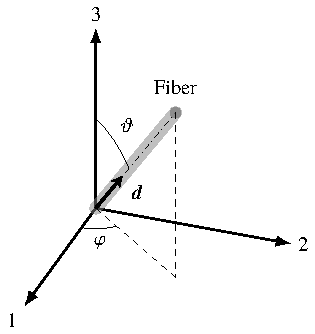
\includegraphics[scale=0.8]{direction_vector}
	\caption{Representation of direction vectors in $\mathbb{S}^2$}
	\label{fig:direction_vector}
\end{figure}%



	
	Generally, the continuous orientation PDF can be approximated in the case of $N$ discrete non-zero values of the oriented function $f(\tena{d})$ by an empirical distribution density in the form~\autocite{Kanatani.1984}
	\begin{equation}
		\psi(\tena{d})=\frac{1}{N}\sum_{j=1}^N\delta(\tena{d}-\tena{d}^{(j)}),
	\end{equation}
	where by means of the Dirac delta generalised function ($\delta$), the existence of a fibre along a particular direction in $\mathbb{S}^2$ is captured:
	\begin{equation}
		\delta(\tena{d}-\tena{d}^{(j)})= \frac{1}{\sin\vartheta^{(j)}} \delta(\varphi-\varphi^{(j)})\delta(\vartheta-\vartheta^{(j)}).
	\end{equation}
	Thus, the average value obtained from a continuous oriented function in Eq.~\eqref{eq:odist} can be replaced by $N$ contributions from a discretised counterpart:
	\begin{equation}
		\averot{f} =\frac{1}{N}\sum_{j=1}^N f(\tena{d}^{(j)}),
	\end{equation}
	which is equivalent to Kanatani's orientation tensor of first kind~\autocite{Kanatani.1984}. Alternative versions are available in literature; for instance in the context of fibre-reinforced composites, a weighted average is used such that the volume of fibres ($V_\text{f}$) is the scaling parameter~\autocite{Muller.2016}:
	\begin{equation}\label{eq:OTw}
		\averot{f}^\prime =\frac{1}{V}\sum_{j=1}^{N} V^j_\text{f}\; f(\tena{d}^{(j)}),
	\end{equation}
	where $V$ is the total volume of fibres in the sample.
%	This formula can be applied to layers 
%	\begin{equation}
%		\averot{f}_\text{layer} =\frac{1}{V_\text{layer}}\sum_{j=1}^{N_\text{layer}} V_\text{f}\; f(\tena{d}^{(j)}),
%	\end{equation}	
%	where $V_\text{layer}$ is the volume of the layer and $N_\text{layer}$ is the number of fibres per layer. Herein, per-element normalisation is applied:
%	\begin{equation}
%		\averot{f}_\text{element} =\frac{1}{V_\text{element}}\sum_{j=1}^{N_\text{fiber/element}} V_\text{f}\; f(\tena{d}^{(j)}),
%	\end{equation}
%	where $V_\text{element}$ is the volume of the element and $N_\text{fiber/element}$ is the number of fibres in that element.
\subsection{Averaged Orientation Tensor}
	Defining the \textit{orientation tensor} as
	\begin{equation}
		\tenb{A}\equidef \tena{d}\dyad\tena{d},\label{eq:ot}
	\end{equation}
	results in an \textit{averaged orientation tensor} of order $2k$\footnote{mathematically, it is shown by $\tenn{H}{2k}\equiv\averot{\tena{d}^\tenpow{2k}}$ , and thus it is a tensor of order $2k$.} or orientation tensor of first kind (moment tensor)~\autocite{Kanatani.1984}:
	\begin{equation}
		\ten{H}_k\equidef \averot{\tenb{A}^\tenpow{k}}.\label{eq:ot1}
	\end{equation}
	Since $\tenb{A}$ has no odd powers, it is symmetric, and thus its average $\ten{H}_k$ is also symmetric~\autocite{Kanatani.1984,Comon.2008}. Note that this formulation automatically rules out the trivial odd-ordered combinations of orientation vectors. Moreover, lower order averaged orientation tensors are obtained by contracting higher ones: 
	\begin{equation}
	\ten{H}_{k-1} = \ten{H}_{k}\dscp\unitb,\qquad\qquad \forall k\in\Natural\ge2,
	\end{equation}
	and therefore they are not independent~\autocite{Advani.1987}. This is another incentive to use the orientation tensor of the third kind of various orders since they are independent from each other~\autocite{Kanatani.1984}. Both types are similar, and thus share the same eigenvalues and eigenvectors. Therefore, either one can be used in spectral analysis.
	
	The second-order orientation tensor $\tenb{H}_{1}=\averot{\tenb{A}}$ is frequently used in the literature; for simplicity, it will be denoted by $\tenb{H}$ henceforth. The fourth-order orientation tensor $\tend{H}_{2}=\averot{\tenb{A}\dyad\tenb{A}}$ (denoted by $\tend{H}$) is also available in the literature, see~\autocite{Vasta.2014}. In either case, symmetry reduces the number of independent parameters. For instance in~\autocite{Gasser.2006}, a `generalised structure tensor' is introduced to capture the orientation of collagen fibres in soft tissue (equivalent to the second-order averaged orientation tensor). As mentioned earlier, the orientation PDF is centro-symmetric, and thus $\psi(-\tena{d})=\psi(\tena{d})$. An additional symmetry axis $\tena{d}_0$ could also exist if $\psi(\tenb{Q}\scp\tena{d}_0)=\psi(\tena{d}_0)$, where $\tenb{Q}$ belongs to the symmetry group of all proper orthogonal tensors about $\tena{d}_0$. If it is assumed that the polar axis coincides with $\tena{d}_0$, the averaged orientation tensor can be represented by a single dispersion parameter. In the absence of such symmetry in an $n$-dimensional space, evaluation of the $2k$-order average orientation tensor requires the calculation of $n^{2k}$ integrals over $\mathbb{S}^2$ (without considering its universal symmetry). A $k$-th order averaged orientation tensor can be represented by $k$ scalars provided that a transversely isotropic orientation PDF exists~\autocite{Hashlamoun.2017}.
	 
	%$k_1$:
%	\begin{equation}
%		\tenb{H}=k_1\unitb +(1-3k_1)\tenb{A}_0,
%	\end{equation}
%	where $\tenb{A}_0\equidef\tena{d}_0\dyad \tena{d}_0$ is the orientation tensor with the additional symmetry axis. Consequently, the orientation PDF becomes independent of the polar angle, i.e., $\psi(\vartheta,\varphi)\equiv\psi(\varphi)$. It is shown that the value of the dispersion parameter is readily calculated from
%		\begin{equation}
%			k_1=\pi\int_{0}^{\pi}\psi(\varphi)\sin^3\varphi\;\dif\varphi.
%		\end{equation}
 	Transverse isotropy of the orientation PDF does not exist in most practical cases, at least not globally. For instance in a short FRC, no symmetry groups might be found for the whole specimen or at the other extreme, even a complete isotropy might be detected for completely random samples; either case might be unsophisticated characterisations of meso-structure. On the other hand, a symmetry axis might just exist locally where only a few fibres (ideally one) exist(s) whereas demanding such a condition for the whole sample is a very strong one. The remedy might be an auxiliary map with enough resolution so that our assumption of transverse isotropy carries small errors. In the current study, the resolution of the auxiliary maps is set according to the finite elements of composite. Obviously, other finer/coarser arrangements are possible. 

%	\paragraph{Additive decomposition of orientation tensor} In~\autocite{Shertzer.2011}, the second-order average orientation tensor is additively decomposed to its dilatoric (isotropic or volumetric) and deviatoric (or isochoric) components: 
%	\begin{equation}
%	\tenb{H}_1=\tenb{H}^\vol_1+\tenb{H}^\dev_1.
%	\end{equation}
%	The deviatoric component is identical to Kantani's orientation tensor of third kind. The isotropic component represents the part of averaged orientation tensor that cannot identify any preferred orientation. Thus, meso-structure is deemed isotropic provided that the deviatoric component vanishes. This state is equivalent to having recurring eigenvalues for the orientation tensor. This paragraph is not correct since the orientation tensor of third kind is a traceless symmetrical tensor and the aforementioned additive decomposition does not product such as result. An decomposition into irreducible tensors is required that gives a second-order tensor as the sum of zeroth-, first-, and second-order tensors.
\subsection{Homogenisation}
	\paragraph{Enhanced rule of mixture} Consider a transversely isotropic material with the axis of symmetry along the 1-direction and the 2-3 isotropy plane. From the strength-of-material point of view, homogenisation formulas for unidirectional composites, i.e., the rule of mixture (RoM) and the inverse rule of mixture (IRoM), are based on the iso-strain and iso-stress assumptions, respectively:
	\begin{subequations}
	\begin{alignat}{2}\label{eq:rom}
		E_1 		=\;& \zeta_\text{f}E_\text{f}          &&+\zeta_\text{m}E_\text{m},\\
		\frac{1}{E_2}	=\;& \frac{\zeta_\text{f}}{E_\text{f}} &&+ \frac{\zeta_\text{m}}{E_\text{m}},
	\end{alignat}
	\end{subequations}
	where $\zeta$ is the volume fraction and $E$ shows the elastic modulus. Subscripts of `$\text{f}$' and `$\text{m}$' are used to denote fibre and matrix phases, respectively. The elastic moduli $E_1$ and $E_2$ set the upper and lower bounds of stiffness and are in accordance with the longitudinal and transverse stiffnesses, respectively. An efficiency parameter $\varkappa$ is used to further adjust these bounds by altering the contribution of fibres. The result is the enhanced rule of mixture (En-RoM)~\autocite{Summerscales.2019} 
	\begin{subequations}
	\begin{alignat}{2}
		\hat{E}_1 &= \varkappa\zeta_\text{f}E_\text{f}+\zeta_\text{m}E_\text{m},\label{eq:enrom}\\
		\frac{1}{\hat{E}_2} &=\frac{\zeta_\text{f}}{\varkappa_\text{a} E_\text{f}}+ \frac{\zeta_\text{m}}{E_\text{m}},\label{eq:enirom}
	\end{alignat}
	\end{subequations}
	with $\varkappa \equidef \varkappa_\text{a}\varkappa_\text{d}\varkappa_\text{l}\varkappa_\text{o}$ where $\varkappa_\text{a}$ is the fibre area correction factor (FACF), $\varkappa_\text{d}$ is the fibre diameter distribution factor (FDDF), $\varkappa_\text{l}$ is the fibre length distribution factor (FLDF), and $\varkappa_\text{o}$ is the fibre orientation distribution factor (FODF), respectively. Well-characterised fibre diameters assign a unit value to FDDF; a unit value is also assigned to FLDF since continuous fibres are the focus of the current study. The FODF can be estimated by Krenchel's formula~\autocite{Krenchel.1964}
		\begin{equation}
			\varkappa_\text{o}=\sum_n a_n\cos^4\theta,\label{eq:Krenchel}
		\end{equation}
	where $a_n$ is the fraction of fibres making a $\theta$ angle with the applied load. The FACF is suggested by~\autocite{Virk.2009} and is used to rectify the underestimation of stiffness and strength due to an overestimation in measuring the cross-section area (CSA) of fibres. For jute fibres, a typical value of 1.42 was suggested in the same study. 
	
	In the same spirit, the relation for shear modulus ($\hat{G}_{12}$) is established
	\begin{subequations}
	\begin{alignat}{2}
		\frac{1}{\hat{G}_{12} } &=\frac{\zeta_\text{f}}{\varkappa_\text{a} G_\text{f}}+ \frac{\zeta_\text{m}}{G_\text{m}},\label{eq:enirom2}
	\end{alignat}
	\end{subequations}
	The Poisson's ratio in anisotropic elasticity could be defined as $\nu_{ij}\equidef -\sfrac{\varepsilon_j}{\varepsilon_i}$ and for an orthotropic material, due to the symmetry of the compliance matrix, the relation $ \sfrac{\nu_{ij}}{E_i}  =\sfrac{\nu_{ji}}{E_j}$ is established. The Poisson's ratio of the composite $\nu_{12}$ is obtained from
	\begin{equation}
		\nu_{12}= \zeta_\text{f}\nu_\text{f}+\zeta_\text{m}\nu_\text{m}.\label{eq:enrom2}\\
	\end{equation}
	Finally, the transversely isotropic elastic compliance matrix $\tend{C}^\inv$ for the composite along the $1$-axis, i.e., when 2-3 is the plane of symmetry, is established using contracted Voigt notation:
	\begin{equation}\label{eq:Cinv}
	\mat{C}^\inv=
	\left[
	\begin{array}{cccccc}
		\frac{1}{\hat{E}_1} & -\frac{\nu_{21}}{\hat{E}_2} & -\frac{\nu_{21}}{\hat{E}_2} &            0            &            0            &            0            \\
		                      &       \frac{1}{\hat{E}_2}        & -\frac{\nu_{23}}{\hat{E}_2} &            0            &            0            &            0            \\
		                      &                                   &       \frac{1}{\hat{E}_2}        &            0            &            0            &            0            \\
		                      &                                   &                                   & \frac{1}{\hat{G}_{23}} &            0            &            0            \\
		                      &            \text{sym}             &                                   &                         & \frac{1}{\hat{G}_{12}} &            0            \\
		                      &                                   &                                   &                         &                         & \frac{1}{\hat{G}_{12}}
	\end{array}
	\right],
	\end{equation}		
	where $\hat{G}_{23}=\frac{\hat{E}_2}{2(1+\nu_{23})}$. 
%	The Kelly-Tyson model~\autocite{Kelly.1965} is used to evaluate the strength of unidirectional composites $\sigma^\prime_\text{c}$. Following the approach in extending Eq.~\eqref{eq:rom} to Eq.~\eqref{eq:enrom}, the enhanced Kelly-Tyson model (En-KT) is introduced for natural fibres:
%	\begin{equation}
%		\sigma^\prime_\text{En,c} = \kappa \zeta_\text{f}\sigma^\prime_\text{f}+\zeta_\text{m}\sigma^*_\text{m},\label{eq:en-KT}
%	\end{equation}
%	where $\sigma^\prime_\text{f}$ is the strength of fibre, and $\sigma^*_\text{m}$ is the stress in the matrix at composite failure---assuming a dominant fibre failure mechanism, i.e., the matrix is more compliant compared to the fibre under iso-strain conditions. This estimate is used to check the failure of the homogenised elements. 
	
	Equations~\eqref{eq:enrom} to \eqref{eq:enrom2} are generally used globally and in order to apply them locally, the efficiency parameter and the volume fraction must be localised. The volume fraction is readily calculated from its auxiliary map and all of the parameters involved in calculation of efficiency parameter $\varkappa$ can be assumed constant except for the FODF since its spatial variation is not negligible---specially in the cases where fibre clustering or resin-rich volumes exist. Thus, the second auxiliary map would be that of the orientation tensor. 
		
	Using the obtained material properties, the elastic tensor for a transversely isotropic material is in hand. The axis of symmetry is obtained from the spectral analysis of the orientation tensor, i.e., the principal direction of the material is denoted by the eigenvector of the maximum eigenvalue of the orientation tensor. This tensor is used to calibrate the more general formulation discussed in the following section.
	
	
%	An alternative to the global formulation is using Krenchel's formula in Eq.~\eqref{eq:Krenchel} 
%			 the FODF is calculated in two ways: either replaced by the local orientation tensor, or calculated using the global overall orientation of the spectral analysis.
%		
	
	
	

%	The use of 2D embedded fibre elements artificially increases the volume of the matrix since in the fibre-occupied volume, matrix still exists. Thus, this should be considered in the calculations. This can be done either by modifying the elastic moduli or applying a correction factor to the volume of the matrix, e.g., by reducing the overall thickness of the composite.

\subsection{Constitutive Material Model}	
	In~\autocite{Spencer.1984}, the formulation of elastic moduli of composites was carried out by setting up a quadratic free energy function in which the invariants of the orientation tensor $\tenb{H}$ and infinitesimal strains tensor $\tenb{\epsilon}$ were incorporated. The result is rearranged in the following (minor and major) symmetric form for the averaged elastic tensor:
	\begin{equation}\label{eq:C}
	\averot{\tend{C}} = 3\lambda\unitd^\vol+2G_\text{T}\unitd^\sym +2\alpha (\tenb{H}\dyad\unitb)^\sym+4(G_\text{L}-G_\text{T})(\tenb{H}\dyadd\unitb)^\sym +\beta\tend{H},
	\end{equation}
	where out of the five constants, $\lambda$, $\alpha$, and $\beta$ are functions of elastic properties of an aligned FRC and $G_\text{L}$ and $G_\text{T}$ are its shear moduli in the longitudinal and transverse directions. All these parameters are calculated based on the relations of the previous section. The orientation tensor adjusts the deviation from this perfectly aligned status. Overall, the symmetry group of this constitutive tensor is all the orthogonal transformations about the axis of symmetry. This form is identical to what is proposed in~\autocite{Advani.1987} or more generally in~\autocite{Cowin.1985}. Herein, the rearranged representation concisely illustrates the individual symmetrical terms in direct notation. Furthermore, the 4th-order averaged orientation tensor $\tend{H}$ can be replaced by means of various closure approximations; see~\autocite{Breuer.2019,Advani.1990}.% the last term is replaced by a quadratic approximation, . Herein, a quadratic approximation is used; see~\autocite{Breuer.2019}.

	Considering the fact that the invariant $\tr(\tenb{H})$ is unit, the model in Eq.~\eqref{eq:C} is calibrated for the principal material directions. This is the case where symmetry reduces the the number of independent parameters to one. Namely, the only non-zero component of $\tenb{H}$ becomes its maximum eigenvalue. Thereby, the constitutive equation of transversely isotropic material becomes available for any arbitrary orientation tensor. Accordingly, the material parameters of Eq.~\eqref{eq:C} can be readily related to the Voigt components of the elastic tensor in the principal direction---which is obtained by inverting Eq.~\eqref{eq:Cinv}:
	\begin{subequations}
%	\begin{alignat}{2}
%		B_1\equiv&\;\beta  			&&= C_{11}+C_{22}-2C_{12}-4C_{66},\\
%		B_2\equiv&\;\alpha &&=C_{12}-C_{23},\\
%		B_3\equiv&\;\mu_\text{LL}-\mu_\text{TL}&&=C_{66}+0.5(C_{23}-C_{22}),\\
%		B_4\equiv&\;\lambda&&=C_{23},\\
%		B_5\equiv&\;\mu_\text{TL}&&=0.5(C_{22}-C_{23}).
%	\end{alignat}
	\begin{alignat}{2}
		\beta  	&= C_{11}+C_{22}-2C_{12}-4C_{66},\\
		\alpha  &=C_{12}-C_{23},\\
		G_\text{L}-G_\text{T}&=C_{66}+\half(C_{23}-C_{22}),\\
		\lambda&=C_{23},\\
		G_\text{T}&=\half(C_{22}-C_{23}),
	\end{alignat}
	\end{subequations}	
	where $G_\text{T}\equiv \hat{G}_{23}$ and $G_\text{L}\equiv \hat{G}_{12}$ retain their physical meanings.

	After incorporating the averaged orientation tensor, an explicit formulation of the final elasticity tensor for any arbitrary orientation can be obtained from Eq.~\eqref{eq:C}. By assuming $\nu_\text{23}= 0$ and a planar distribution of fibres on the 1-2 plane, the non-zero components of the elastic tensor become
	\begin{subequations}
	\begin{alignat}{2}
		C_{11}=\;&\lambda + 2G_\text{T} + 4(\half\alpha+G_\text{L}-G_\text{T})H_{11}+\beta H_{11}^2,\\
		C_{12}=\;&\lambda +\alpha(H_{11}+H_{22})+\beta H_{11}H_{22},\\
		C_{13}=\;&\alpha H_{11}+\lambda,\\
		C_{16}=\;&\alpha H_{11} + (\alpha+2G_\text{L}-2G_\text{T})H_{12}+\beta H_{11}H_{12},\\
		C_{22}=\;&\lambda + 2G_\text{T} + 4(\half\alpha+G_\text{L}-G_\text{T})H_{22}+\beta H_{22}^2,\\
		C_{23}=\;&\alpha H_{22}+\lambda,\\
		C_{26}=\;&\alpha H_{22} + (\alpha+2G_\text{L}-2G_\text{T})H_{12}+\beta H_{22}H_{12},\\
		C_{33}=\;& \lambda + 2G_\text{T},\\
		C_{36}=\;& \alpha H_{12},\\
		C_{44}=\;& (G_\text{L}-G_\text{T})H_{22}+G_\text{T},\\
		C_{45}=\;& (G_\text{L}-G_\text{T})H_{12},\\
		C_{55}=\;& \beta H_{12}^2 (G_\text{L}-G_\text{T})(H_{11}+H_{22})+G_\text{T},\\
		C_{66}=\;&G_\text{T} + (G_\text{L}-G_\text{T})(H_{11}+H_{22})+\beta H_{12}^2.
	\end{alignat}
	\end{subequations}
	The plane stress case governs the behaviour of thin laminates and is of interest in the current study. Therefore, the reduced stiffness elastic tensor ($\tilde{\mat{C}}$)~\autocite{Herakovich.1998,Altenbach.2010c} can be calculated from the evaluated components:	
	\begin{equation}\label{eq:plane}
	\tilde{\mat{C}}_{\text{2D}}=
	\left[
		\begin{array}{ccc} 
			\tilde{C}_{11}  & \tilde{C}_{12} & \tilde{C}_{16}\\
					& \tilde{C}_{22} & \tilde{C}_{26}\\
			\text{sym}		&		 & \tilde{C}_{66}\\
		\end{array}	
	\right],
	\end{equation}
	with 
	\begin{equation}
	\tilde{C}_{ij}\equidef C_{ij}-\frac{C_{i3}C_{3j}}{C_{33}},\qquad\qquad\forall i,j\in\{1,2,6\}.
	\end{equation}

\begin{comment}

\subsection{Generalised Rule of Mixture}
	In order to generalise the enhanced rule of mixture (En-RoM)~\autocite{Summerscales.2019}, the fibre efficiency parameter ($F$) is introduced:
	\begin{equation}
		f \equidef \kappa\eta_\text{d}\eta_\text{l}\eta_\text{o},
	\end{equation}
	where $\kappa$ is the fibre area correction factor (FACF), $\eta_\text{d}$ is the fibre diameter distribution factor (FDDF), $\eta_\text{l}$ is the fibre length distribution factor (FLDF), and $\eta_\text{o}$ is the fibre orientation distribution factor (FODF), respectively. Herein, FODF is dropped since orientation tensors are used in a local sense. Also well-characterised fibre diameters assign a unit value to FDDF; a unit value is also assigned to FLDF, and thus the effective elastic tensor of fibres is readily amended:
	\begin{equation}
		\tend{C}^{\text{(f)}} \equidef \kappa\hat{\tend{C}}^\text{(f)}.
	\end{equation} 
	% TODO check the first citation and find the second citation
	%	TECHNICAL MISTAKE.		folllowing paragraph is removed.
	%	Furthermore, in the case of using embedded fibres, parametric studies show that the nominal and true volume fractions result in different responses especially in higher volume fractions~\autocite{Javanbakht.2016b}. Thus, this discrepancy is compensated by modifying either the thickness of the model composite or its material properties~\autocite{}. In the sprite of En-RoM, the model correction factor $m$ is applied:
	%	\begin{equation}
	%		\tend{C}^{\text{(m)}} \equidef m\,\hat{\tend{C}}^\text{(m)},
	%	\end{equation}		
	%	which can be interpreted as reducing the efficiency of the matrix ($\eta_\text{m}<1$).
	
	In mean-field methods, the volume averaging of an arbitrary field ($\tend{T}$) over the $\Omega$ domain is defined as
	\begin{equation}
	\avevol{\tend{T}} \equidef \int_{\Omega}\tend{T}(\tena{x})\dif\Omega,
	\end{equation}
	where $\tena{x}$ is the position vector. In a biphasic material, the domain consists of fibre (f) and matrix (m) volumes, i.e., $\Omega_\text{f} \cup \Omega_\text{m}=\Omega$ and $\Omega_\text{f} \cap \Omega_\text{m}=\varnothing$. To set up the micro-mechanical formulation for a multi-phase continuum, the micro-constitutive relation between the stress and strain of the $p$ phase is
	\begin{alignat}{2}
	\tenb{\sigma}^\text{(p)} &= \tend{C}^\text{(p)}\dscp\tenb{\epsilon}^\text{(p)},\qquad\qquad\forall\text{p}\in\{\text{f},\text{m}\},
	\end{alignat}
	where $ \tend{C}^\text{(p)}$ is the elastic stiffness of the phase $\text{p}$. The averaged macro-constitutive relation for the homogenised medium is
	\begin{alignat}{2}
		\avevol{\tenb{\sigma}} &= \tend{C}\dscp\avevol{\tenb{\epsilon}},
	\end{alignat}
	where $\tend{C}$ is the effective elastic stiffness of the multi-phase medium. The average stress and average strain of the medium are $\avevol{\tenb{\epsilon}}=\sum\zeta^{(p)}\tenb{\epsilon}^{(p)}$ and $\avevol{\tenb{\sigma}}	=\sum\zeta^{(p)}\tenb{\sigma}^{(p)}$ where $\zeta^{(p)}=\sfrac{\Omega_\text{p}}{\Omega}$ is the volume fraction of the $p$ phase. In the next step, localisation tensors~\autocite{Hill.1963} are used to relate the overall averaged properties to the phase-averaged ones:
	\begin{alignat}{2}
	\forall\text{p}\in\{\text{f},\text{m}\}:\left\{
	\begin{array}{rl}
		\avevol{\tenb{\epsilon}}^\text{(p)} &= \tend{A}^\text{(p)}\dscp\avevol{\tenb{\epsilon}},\\[0.2cm]
		\avevol{\tenb{\sigma}}^\text{(p)} 	&= \tend{A}^\text{(p)}\dscp\avevol{\tenb{\sigma}}.
	\end{array}\right.,
	\end{alignat}
	and obtain the effective elastic tensor
	\begin{equation}
	\tend{C}=\sum_\text{(p)}\zeta^\text{(p)} \tend{A}^\text{(p)}\dscp\tend{C}^\text{(p)}.
	\end{equation}
	Adopting Voigt's assumption demands $ \avevol{\tenb{\epsilon}^\text{(f)}}\equimust\avevol{\tenb{\epsilon}^\text{(m)}}\equimust\avevol{\tenb{\epsilon}}$ that results in $\sum_\text{(p)}\zeta^{(p)}\tend{A}^\text{(p)}=\unitd^\sym$. Finally, the general form of rule of mixture for a bi-phasic medium is obtained
	\begin{equation}
	\tend{C}=\sum_\text{(p)}\zeta^\text{(p)}\tend{C}^\text{(p)}.
	\end{equation}


	
	%TODO non-local formulation
	%	Setting up a local model might result in very localised behaviour when softening behaviour is involved. One remedy is to use a non-local scheme by replacing the local strain field by its weighted average, which requires introducing a length parameter ($\ell$). So in the current model, the orientation is localised while the non-local strain field is used.

\subsection{Spectral Decomposition}
	In the principal coordinates and in the most general case, the second order orientation tensor reduces to three distinct eigenvalues: $\lambda_\text{max}$, $\lambda_\text{int}$, and $\lambda_\text{min}$. Due to the negligible out-of-plane orientation of fibres, especially for laminar meso-structures, the minimum eigenvalue vanishes, i.e., $\lambda_\text{min}=0$. Moreover, since $\tr{\tenb{H}}=1$, the the second-order average orientation tensor decomposes to:
	\begin{equation}
		\tenb{H}=\lambda_\text{max}\base^\prime_1\dyad\base^\prime_1+(1-\lambda_\text{max})\base^\prime_2\dyad\base^\prime_2,
	\end{equation}
	where $\base^\prime_1$ is assumed to be the averaged preferred direction of the fibres. 
	
	Rotation about an arbitrary fixed axis, denoted by the direction vector $\tena{m}$, is carried out by the proper unimodular rotation tensor~\autocite{Eremeyev.2013}:
	\begin{equation}
		\tenb{R}_{\scriptsize\tena{m}}(\alpha)=\tena{m}^\tenpow{2}+\cos\alpha(\unitb-\tena{m}^\tenpow{2})-\sin\alpha\;\tena{m}\cross\unitb,
	\end{equation}
	where $\alpha$ is the rotation angle about the axis. Note that the first term is the projection tensor along the axis $\tena{m}$, the second term is the projection tensor over the corresponding plane of the axis, and the third term represents a skew-symmetric second-order tensor.
	
	Assume an arbitrary direction denoted by direction vector $\tena{a}_0$ that makes an angle $\alpha_0=\cos^{-1}(\tena{a}_0\scp\base^\prime_1)$ with the maximum principal direction of $\tenb{H}$. Rotation of $\tenb{H}$ from principal direction is carried out by $\tenb{R}_{\scriptsize\tena{m}_0}(\alpha_0)\Rayleigh\tenb{H}$ where $\tena{m}_0=\frac{\tena{a}_0\cross\base^\prime_1}{\norm{\tena{a}_0\cross\base^\prime_1}}$ is the axis of rotation.

\subsection{Direction-dependent Elastic and Bulk Moduli}
	The direction-dependent elastic modulus 
	\begin{equation}
		E(\tena{d})=(\tena{d}^\tenpow{2}\dscp\tend{C}^\inv\dscp\tena{d}^\tenpow{2})^\inv,
	\end{equation}
	and the direction-dependent bulk modulus
	\begin{equation}
		K(\tena{d})=\frac{1}{3}(\unitb\dscp\tend{C}^\inv\dscp\tena{d}^\tenpow{2})^\inv,
	\end{equation}
	are evaluated with respect to the fixed arbitrary direction $\tena{d}$ where $\tend{C}^\inv$ is the elastic compliance tensor.



% --------------------------------------------------------------------------------------------------
\subsection{Representing the Elastic Stiffness of the Composite}
	The response of the composite is equivalent to the contributions from the isotropic matrix, isotropic fibres, and anisotropic fibres (considered by means of the orientation tensor).



	
\subsection{Formulation In Terms of Projectors}
	In a transversely isotropic materials the normal of the isotropic transverse plane denotes the axis of symmetry (along the axial direction). The introduced orientation tensor ($\tenb{A}$) can be regarded as a projector along the axial direction. By adding the projector of the transverse plane ($\tenb{T}$), a complete projector set is obtained:
	\begin{alignat}{2}
		\tenb{A}\equidef\; &\tena{d}\dyad\tena{d},\tag{\ref{eq:ot} revisited}\\
		\tenb{T}\equidef\; &\unitb - \tenb{a}
	\end{alignat}
	where the bi-orthogonality ($\tenb{A}\scp\tenb{T}=\tenb{T}\scp\tenb{A}=\nullb$) and idempotency ($\tenb{A}^n=\tenb{A}$ and $\tenb{T}^n=\tenb{T}$) of the projectors are satisfied.
	
\subsection{Plane Strain Formulation}	
	In this section, the general formula is reduced to the simple plane strain case. The orientation PDF becomes independent of the polar angle, i.e., $\psi(\vartheta,\varphi)\equiv\psi(\varphi)$.




\subsection{Matrix Representation of a General 4th-order Tensor}
	Often in order to carry out numerical analysis, the matrix presentation of tensors is required. For instance, general second- and fourth-order tensors can be arranged in terms of $3\times 3$ matrices (or $9\times 1$ column vectors) and $9\times 9$ matrices (or $81\times 1$ column vectors), respectively. Similarly, all tensorial operations should be translated to the algebra of matrices.


\subsection{Matrix Representation of Elastic Tensor}
	Fedorov's~\autocite{Fedorov.1968} representation of the elastic tensor $\tend{C}$ is obtained by using the orthonormal basis
	\begin{subequations}
	\begin{alignat}{2}
		\tena{e}^\prime_1\equidef&\;&         \base_1\dyad&\base_1,\\
		\tena{e}^\prime_2\equidef&\;&         \base_2\dyad&\base_2,\\
		\tena{e}^\prime_3\equidef&\;&         \base_3\dyad&\base_3,\\
		\tena{e}^\prime_4\equidef&\;&\sqrt{2}(\base_2\dyad&\base_3)^\sym,\\
		\tena{e}^\prime_5\equidef&\;&\sqrt{2}(\base_1\dyad&\base_1)^\sym,\\
		\tena{e}^\prime_6\equidef&\;&\sqrt{2}(\base_1\dyad&\base_1)^\sym,
	\end{alignat}
	\end{subequations}
	to obtain an equivalent six-by-six elasticity matrix $\mat{C}$:
	\begin{equation}\label{eq:fedorov}
		\mat{C}_{ij} \equidef 	\tena{e}^\prime_i\scp\tend{C}\scp\tena{e}^\prime_j\qquad\qquad\forall i,j\in\{1,2,...,6\}.
	\end{equation}
	This matrix representation results in the following form of generalised Hooke's law:
	
	Note that Eq.~\eqref{eq:fedorov} is bridging between the tensorial and matrix notations. The introduced basis vectors are to ensure the equivalence between the following tensorial and matrix operations~\autocite{Nordmann.2018}:
	
	
	For the case of transversely isotropic material (hexagonal crystals), 5 material parameters plus the axis of symmetry must be known~\autocite{Bohlke}.
	
\subsection{Anisotropy measures}
	
	 
\subsection{Creating an observation mesh}
	If a $m\times n$ uniform mesh is used for the FE analysis, the same mesh could be used to monitor the orientation of elements. 
	


\pagebreak
% --------------------------------------------------------------------------------------------------
\subsection{Anisotropic Failure Criterion}
	A general failure criterion for anisotropic materials can take the following form~\autocite{Goldenbart}:
	\begin{equation}%TODO by adding a contraction operator and a sigma this can be more compact
		f\equidef \sum_{k=1}^{n}
		(\tenb{\sigma}^\tenpow{k}\contract\tenn{S}{2k})^{\alpha_k} \le 1,\qquad\qquad \alpha_k \in \Real,		
%		(\tenb{\sigma}\dscp\tenb{S})^\alpha + (\tenb{\sigma}^\tenpow{1}\contract\tend{S})^\beta +
%		(\tenb{\sigma}^\tenpow{2}\contract\tenn{S}{6})^\gamma + \ldots\le 1,\qquad\qquad \alpha, \beta, \gamma, ... \in \Real,
	\end{equation}
	where Cauchy stress tensor ($\tenb{\sigma}$), and strength tensors ($\ten{S}$) are related via the scalars ($\alpha_k$). By choosing the appropriate scalars and the order of tensors, other similar failure criteria are obtained. For instance, Tsai-Wu criterion~\autocite{Tsai.1971} is a special case for which the linear and quadratic terms are used~($\alpha_1=\alpha_2=1$), i.e., the linear combination of first and second order tensors:
	\begin{equation}
		f_\text{Tsi-Wu}\equidef \tenb{\sigma}\dscp\tenb{S} + (\tenb{\sigma}\dyad\tenb{\sigma})\contract\tenn{S}{4} =\tenb{\sigma}\dscp\tenb{S} + \tenb{\sigma}\dscp\tend{S}\dscp\tenb{\sigma}^\tran.
	\end{equation}	 

	
	A scalar-valued function of Cauchy stress tensor ($\tenb{\sigma}$), orientation tensor ($\tenb{H}$) and fibre volume fraction ($v_\text{f}$) is assumed~\autocite{Cowin.1986}:
	\begin{equation}
		f\equiv f(\tenb{\sigma}, \tenb{H}, v_\text{f}).
	\end{equation}
	Since the anisotropy of the continuum is incorporated by means of the orientation tensor, $f$ must succumb to every symmetry, i.e., it must satisfy the isotropy condition:
	\begin{equation}
		f(\tenb{\sigma}, \tenb{H}, v_\text{f})\equimust f(\tenb{Q}\Rayleigh\tenb{\sigma}, \tenb{Q}\Rayleigh\tenb{H}, v_\text{f}),
	\end{equation}
	where $\tenb{Q}$ is the orthogonal rotation tensor. Alternative to satisfying this equation, a form-invariant anstaz could be considered by including all the invariants of the parameters in the function~\autocite{Boehler.1987}:
	\begin{equation}
		f\equiv f\big(
		\tr{\tenb{\sigma}},\tr{\tenb{\sigma}^2},\tr{\tenb{\sigma}^3},
		\tr{\tenb{H}},\tr{\tenb{H}^2},\tr{\tenb{H}^3},
		\tr{(\tenb{\sigma}\scp\tenb{H})},\tr{(\tenb{\sigma}\scp\tenb{H}^2)},\tr{(\tenb{\sigma}^2\scp\tenb{H})},\tr{(\tenb{\sigma}^2\scp\tenb{H}^2)},v_\text{f}\big).
	\end{equation}
	where $\tr{(\square)}\equidef\tenb{I}\dscp\square$ indicates the trace operator.	
	\begin{equation}
		\tenb{S} =\;g_1\unitb+g_2\tenb{H}+g_3\tenb{H}\scp\tenb{H}
	\end{equation}	
	\begin{alignat}{5}
		\tend{S} =\;&&	f_1 \unitd^\vol 
					&+&f_2 (\tenb{H}\dyad\unitb)^\sym 
					&+&f_3 (\tenb{H}\scp\tenb{H}\dyad\unitb)^\sym\\\nonumber
					&+&f_4 (\tenb{H}\dyad\tenb{H})
				    &+&f_5 (\tenb{H}\scp\tenb{H}\dyad\tenb{H})^\sym 
					&+&f_6 (\tenb{H}\scp\tenb{H}\dyad\tenb{H}\scp\tenb{H})^\sym \\\nonumber
					&+&f_7 \unitd^\sym
					&+&f_8 \big[(\tenb{H}\dyadu\unitb)^\sym + (\unitb\dyadu\tenb{H})^\sym\big]
					&+&f_9 \big[(\tenb{H}\scp\tenb{H}\dyadu\unitb)^\sym + (\unitb\dyadu\tenb{H}\scp\tenb{H})^\sym\big].
	\end{alignat}
% not sure about these parameters. If they are the same parameters as those of the elastic stiffness tensor, the following equations are correct.
%	where
%	\begin{alignat}{5}
%		f_i\equiv f_i(\tr{\tenb{H}},\tr{\tenb{H}^2},\tr{\tenb{H}^3},v_\text{f})\qquad\qquad\forall i\in\{1,...,9\}.
%	\end{alignat}		


\subsection{Anisotropic Failure Criterion}


	Shear strength of composite is assumed to be near

	A general failure criterion for anisotropic materials can take the following form~\autocite{Goldenblat.1966}:
	\begin{equation}
		% Original expanded form:
		%(\tenb{\sigma}\dscp\tenb{S})^\alpha + (\tenb{\sigma}^\tenpow{1}\contract\tend{S})^\beta +(\tenb{\sigma}^\tenpow{2}\contract\tenn{S}{6})^\gamma + \ldots\le 1,\qquad\qquad \alpha, \beta, \gamma, ... \in \Real,
		% is expressed in a more compact way:
		f\equidef \sum_{k=1}^{n}
		(\tenb{\sigma}^\tenpow{k}\contract\tenn{S}{2k})^{\alpha_k} \le 1,\qquad\qquad \alpha_k \in \Real,
	\end{equation}
	where Cauchy stress tensor ($\tenb{\sigma}$), and strength tensors ($\ten{S}$) are related via the scalars ($\alpha_k$). Full contraction ($2k$-times here) is denoted by the $\contract$ symbol. The advantage of this mathematical form is that odd and even terms naturally appear, and thus the strength in compression and tension can be distinguished. This facility is not available in criteria with only quadratic terms, e.g., Tsai-Hill. Therefore, this form could be regarded as a more general criterion with which other more restricted failure criteria are obtained by choosing the appropriate scalars and order of tensors. For instance, Tsai-Wu criterion~\autocite{Tsai.1971} is a special case for which the linear and quadratic terms are used~($\alpha_1=\alpha_2=1$), i.e., the linear combination of first and second order tensors:
	\begin{equation}
		f_\text{Tsi-Wu}\equidef \tenb{\sigma}\dscp\tenb{S} + (\tenb{\sigma}\dyad\tenb{\sigma})\dscp\dscp\tenn{S}{4} =\tenb{\sigma}\dscp\tenb{S} + \tenb{\sigma}\dscp\tend{S}\dscp\tenb{\sigma}^\tran.
	\end{equation}	 
	
	A scalar-valued function of Cauchy stress tensor ($\tenb{\sigma}$), orientation tensor ($\tenb{H}$) and fibre volume fraction ($v_\text{f}$) is assumed~\autocite{Cowin.1986}:
	\begin{equation}
		f\equiv f(\tenb{\sigma}, \tenb{H}, v_\text{f}).
	\end{equation}
	Since the anisotropy of the continuum is incorporated by means of the orientation tensor, $f$ must succumb to every symmetry, i.e., it must satisfy the isotropy condition:
	\begin{equation}
		f(\tenb{\sigma}, \tenb{H}, v_\text{f})\equimust f(\tenb{Q}\Rayleigh\tenb{\sigma}, \tenb{Q}\Rayleigh\tenb{H}, v_\text{f}),
	\end{equation}
	where $\tenb{Q}$ is the orthogonal rotation tensor. Alternative to satisfying this equation, a form-invariant anstaz could be considered by including all the invariants of the parameters in the function~\autocite{Boehler.1987}:
	\begin{equation}
		f\equiv f\big(
		\tr{\tenb{\sigma}},\tr{\tenb{\sigma}^2},\tr{\tenb{\sigma}^3},
		\tr{\tenb{H}},\tr{\tenb{H}^2},\tr{\tenb{H}^3},
		\tr{(\tenb{\sigma}\scp\tenb{H})},\tr{(\tenb{\sigma}\scp\tenb{H}^2)},\tr{(\tenb{\sigma}^2\scp\tenb{H})},\tr{(\tenb{\sigma}^2\scp\tenb{H}^2)},v_\text{f}\big).
	\end{equation}
	where $\tr{(\square)}\equidef\tenb{I}\dscp\square$ indicates the trace operator.	
	\begin{equation}
		\tenb{S} =\;g_1\unitb+g_2\tenb{H}+g_3\tenb{H}\scp\tenb{H}
	\end{equation}	
	\begin{alignat}{5}
		\tend{S} =\;&&	f_1 \unitd^\vol 
					&+&f_2 (\tenb{H}\dyad\unitb)^\sym 
					&+&f_3 (\tenb{H}\scp\tenb{H}\dyad\unitb)^\sym\\\nonumber
					&+&f_4 (\tenb{H}\dyad\tenb{H})
				    &+&f_5 (\tenb{H}\scp\tenb{H}\dyad\tenb{H})^\sym 
					&+&f_6 (\tenb{H}\scp\tenb{H}\dyad\tenb{H}\scp\tenb{H})^\sym \\\nonumber
					&+&f_7 \unitd^\sym
					&+&f_8 \big[(\tenb{H}\dyadu\unitb)^\sym + (\unitb\dyadu\tenb{H})^\sym\big]
					&+&f_9 \big[(\tenb{H}\scp\tenb{H}\dyadu\unitb)^\sym + (\unitb\dyadu\tenb{H}\scp\tenb{H})^\sym\big].
	\end{alignat}
% not sure about these parameters. If they are the same parameters as those of the elastic stiffness tensor, the following equations are correct.
%	where
%	\begin{alignat}{5}
%		f_i\equiv f_i(\tr{\tenb{H}},\tr{\tenb{H}^2},\tr{\tenb{H}^3},v_\text{f})\qquad\qquad\forall i\in\{1,...,9\}.
%	\end{alignat}	
\end{comment}


\section{Methodology}
	\paragraph{Experimental values} Experimental data of jute-fibre reinforced epoxy tensile samples tested in~\autocite{Virk.2011,Virk.2013} are used as a study case. The composite samples were made from a $150\times25\times3.52\,\text{mm}^3$ plate with an average volume fraction of $\zeta_\text{f}=18.88\%$. The average properties of tensile samples were deemed to represent those of the laminate, and thus only the plate properties were used in numerical procedures. The statistical distribution of the fibre orientation, length, and CSA were available in the mentioned studies, see Table~\ref{table:mech} for a summary. The computational analyses were facilitated by means of the interaction between an in-house computer program and a commercial FE package.

	\begin{table}[!h]
	\centering\small
	\caption{Summary of the case study material properties based on the experimental data of~\autocite{Virk.2013,Virk.2016}}\label{table:mech}
	\begin{tabular}{p{0.09\textwidth}p{0.28\textwidth}p{0.475\textwidth}}
	\toprule
	\bfs{Material} 	& \bfs{Parameter} 	& \bfs{Value}\\
	\toprule
	Jute fibre	%	& Constitutive law				& Linear elastic, isotropic\\
					& Axial elastic modulus				& $27.9$ GPa \\
					& Axial-radial Poisson's ratio				& $0.35$ \\
%					& Failure criterion				& Maximum normal stress \\
					& Average axial fibre strength$^\dagger$ & 298.13\, MPa\\
					& Fibre length distribution			& Log-normal (mean=4.183, $\text{SD}=0.976$)\\%(mean=65.6, STD=2.65)\\
					& CSA distribution				& Log-normal (mean=7.55, $\text{SD}=0.52$)\\%(mean=1900.74, STD=1.682)\\
					& Orientation distribution		& Gaussian (mean=7.36, SD=17.95) \\
					& Mean fibre orientation factor & $0.81\pm0.06$\\\midrule
	Epoxy		%	& Constitutive law				& Linear elastic, isotropic\\
					& Elastic modulus				& $2.65$ GPa \\
					& Poisson's ratio				& $0.35$ \\
					& Failure strength				& $61$ MPa\\
					\midrule
	\multicolumn{3}{l}{$^\dagger$ The average axial strength corresponds to a fibre with average length in the distribution.}\\\bottomrule
	\end{tabular}
	\end{table}

	\paragraph{Python pre-processor} In order to avoid modelling discrete fibres, the derived analytical formulation in the previous section is combined with finite element analyses~\autocite{Oechsner.2016}. The object-oriented programming paradigm is used within a Python script to generate pseudo-random long fibres that follow certain distributions. The auxiliary maps were obtained from the generated objects using a python script with multi-processing capability to increase computational efficiency. The FE prototypes were generated using the same Python script through an automated process that managed the parametric model generation from the prototype and controlled the job submissions~\autocite{Javanbakht.2016}. 

	\paragraph{FORTRAN processor} The semi-open MARC/MENTAT 2019 FE package is used to take advantage of its customised subroutine capability~\autocite{Javanbakht.2017}. Namely, the material constitutive behaviour and element strength checking were carried out by means of several FORTRAN90 subroutines. The required auxiliary maps were passed from the Python script to FORTRAN subroutines by means of several data files. The maximum stress failure criterion is used to check the failure of the homogenised medium, i.e., a simultaneous failure of matrix and fibre is simulated. To this end, at the end of every increment, the mean stress of an element was calculated by averaging the stresses at its integration points and compared with the average strength of the element. In the case of failure, the respective element is removed to implicitly incorporate the stiffness reduction effect of damage progression into the FE prototype. The load increments continued until sample failure, which is marked by the solver losing convergence.  

	\paragraph{Python post-processor} The Python script interacted with the MENTAT pre-processor for model generation and then submitted the job to the MARC solver for analysis where FORTRAN subroutines were involved. Afterwards, the script gains the control back and the post-processing result are exported to Excel files. 

	\paragraph{Fibres} Rather than using discrete fibres in the FE model, the auxiliary maps for the local volume fraction and local orientation tensors were used in constitutive modelling. The maps were extracted based on the generated fibre data, i.e., fibre length distribution, fibre CSA distribution, and fibre orientation distribution. The technical jute fibres were assumed to be straight entities with a constant CSA per fibre that were generated from a log-normal distribution of the `true' fibre CSA~\autocite{Virk.2010b}. The quasi-unidirectional fibre orientation distribution was achieved by following a Gaussian distribution of angles and allowing fibres to penetrate the soft boundary of the model to create a periodic structure. The properties of the jute fibres follow the data in Table~\ref{table:mech}. It is worth mentioning that although the length variation of fibres is considered, the variation of length-dependent properties were ignored. For instance, the elastic modulus of fibres was taken to be the mean of the 785 jute samples tested in~\autocite{Virk.2013}, i.e., a mean value of 27.9\,GPa, which is sensibly independent of fibre length. Furthermore, the strength of the fibres was assumed to be length-independent.
%	The true CSA of the fibres was considered by means of the FACF.
		
	\paragraph{Matrix} The epoxy matrix was modelled by 2D plane stress elements (type 3) as an isotropic material. Constitutive material behaviour of the four-node isoparametric quadrilateral elements was replaced by Eq.~\eqref{eq:plane} and linear interpolation functions were used. A perfect bond between the fibres and matrix was assumed, and thus any interphase interactions were disregarded for simplicity.
	
\paragraph{FE prototype} The FE prototype consisted of anisotropic plane stress elements, which represented the homogenised properties of the composite. In order to focus on the effects of orientation, the standard deviation (SD) of the Gaussian orientation distribution was varied from 0 to 20 according to Table~\ref{table:results7}---the $\text{SD}=17.95$ was included for validation against experimental results. Five realisations were created for each SD and the average value of the results were reported in the aforementioned table. In addition to the experimental value, a global method was included.\red~This benchmarking method used the global orientation of the fibres from spectral analysis; then, the FODF was calculated from Eq.\eqref{eq:Krenchel} and substituted into Eq.~\eqref{eq:rom} to obtain the effective elastic modulus.\bl~Moreover, the failure of the homogenised elements were checked and the failed elements removed from the analysis at each increment. The FE analyses halted when achieving convergence became infeasible due to the loss of positive-definiteness of the stiffness matrix.

\red
	\paragraph{Detecting failure} The failure of the homogenised elements were checked by means of the maximum failure stress criterion. At each increment, the three modes of failure in a composite were checked for each element by means of the maximum stress criterion, i.e., fibre failure in tension, matrix failure in tension (in the direction perpendicular to the fibres), and matrix failure in shear. The tensile strength of the composite along the fibres ($\sigma^\prime$) was calculated from the enhanced Kelly-Tyson model (En-KT)~\autocite{Kelly.1965}:
	\begin{equation}
		\sigma^\prime = \kappa_\text{a} \zeta_\text{f}\sigma^\prime_\text{f}+\zeta_\text{m}\sigma^*_\text{m},\label{eq:en-KT_ch10}
	\end{equation}
	where $\sigma^\prime_\text{f}$ is the strength of fibre, and $\sigma^*_\text{m}$ is the stress in the matrix at composite failure. Note that this equation is only applicable to matrices with a higher failure strain than that of the used fibres.
	
	After the strength calculations, the stress tensor was extracted from the integration points of an element and its average value was calculated. From spectral analysis~\autocite{Javanbakht.2017c,Javanbakht.2019}, the principal direction of fibres at the same element was calculated. Knowing the eigen-direction, the average stress tensor was transformed along the fibres and compared against the strength values. According to the weakest link theory, any mode of failure causes the elimination of the element. This procedure was repeated until the termination of the analysis.
\bl

\section{Results and Discussion}
	\paragraph{Mesh density and map resolution} Often, the transfer of data between the FE prototype and the available auxiliary maps is carried out irrespective of the required resolution. Herein, the resolution of these auxiliary maps is linked to the size of elements, i.e., higher mesh densities demand higher resolution from the auxiliary maps. Although in practical cases the resolution might be limited to the accuracy of test apparatus, the approximations above this precision level can be established by the user. Obviously, numerically-generated data can provide the required resolution more easily. In any case, such tensorial fields provide additional information of the meso-structure to obtain better approximations of the response of the heterogeneous medium.

	\begin{figure}[!b]{}
	  	\centering
	  	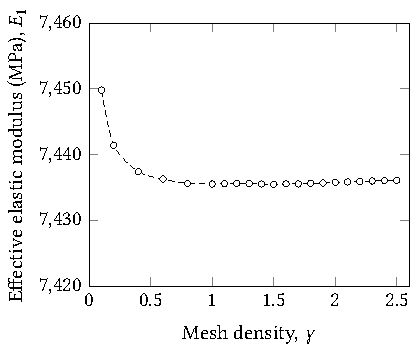
\includegraphics[scale=1]{E_sensitivity}
	%  	\hfil 	\subfloat[][Tensile strength\label{fig:TS_sens}]{\includegraphics[scale=1]{TS_sensitivity}}\\
		\caption{Mesh sensitivity of a local analysis for one realisation ($\text{SD}=20$)}
		\label{fig:mesh_sens}
	\end{figure}%

	\paragraph{Mesh sensitivity} Since element removal has an effect similar to integrating damage into the constitutive material model, mesh dependency inherently exists. Thus, to alleviate this localised deficiency, the elastic modulus of an FE prototype with the highest discrepancy ($\text{SD}=20$) was regarded. Obviously, convergence of other cases with lower SD is obtained more easily. Mesh density is defined as~\autocite{Javanbakht.2016b}
	\begin{equation}
		\gamma\equidef\frac{1}{\ell_\text{mesh}},
	\end{equation}
	where ($\ell_\text{mesh}$) is the mesh length. It is varied over a range of 0.1 to 2 to monitor the convergence behaviour. In the same manner, the auxiliary maps are also refined accordingly. As illustrated in Fig.~\ref{fig:mesh_sens}, the effective (or apparent) elastic modulus of the composite ($E_1$) gains convergence quickly with $\gamma$ over 1. In the current study, a mesh density of 1 is adopted in the analyses considering the trade-off between accuracy and efficiency.

	\paragraph{Refining auxiliary maps} In Fig.~\ref{fig:volfrac_maps}, a fibre volume fraction auxiliary map is shown. The local volume fraction is calculated as a volume average over each element, using Eq.~\eqref{eq:OTw}, and is depicted at its corresponding centre.  Thus, the corner of each pixel in the graphs correspond to the centre of an element. The mesh density controls both the refinement of finite elements and the related auxiliary maps, i.e., finer mesh requires higher resolution auxiliary maps. All the illustrated maps correspond to the same realisation with a fibre volume fraction $\zeta_\text{f}=18.88\%$. It is clear that by increasing the mesh density, a wider range of variation is captured over the domain and a more realistic visualisation of fibre distribution is obtained. 	
	
	A similar argument can be laid out for the fibre orientation distribution. In Fig.~\ref{fig:tensor_maps}, the volume-averaged orientation tensor (weighted by fibre volume) is calculated over each element and depicted along its principal direction. Moreover, the length of each fibre is scaled by the first eigenvalue of the averaged orientation tensor to show the intensity of the anisotropy. In the figures, the angle is scaled 6 times for a better presentation. The mean angle of the ODF is $7.36^\circ$ and SD of 20. It is evident that increasing the resolution of orientation auxiliary map reveals more local fluctuations since the range of angles increase from $7.49^\circ\le \varphi\le 8.17^\circ$ for $\gamma=0.1$ to $3.16^\circ\le \varphi \le13.58^\circ$ for $\gamma=1.5$.


\begin{figure}[!h]{}
  	\centering
	\subfloat[][$\gamma=0.1$\label{fig:TS_sehns}]{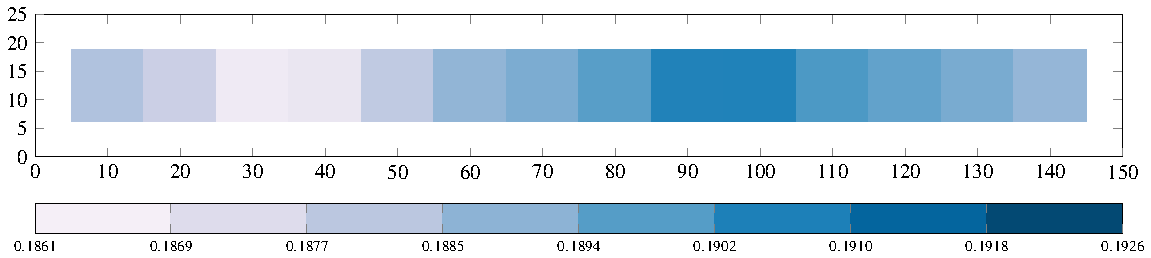
\includegraphics[width=0.9\textwidth]{volfrac_map_md100}}\\
	\subfloat[][$\gamma=0.2$\label{fig:TS_senfs}]{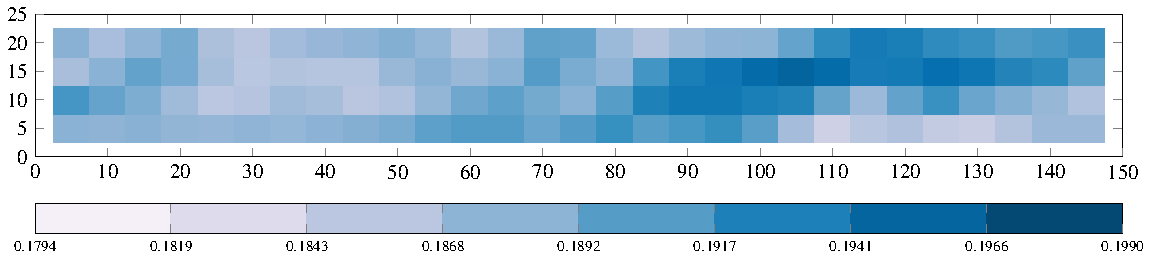
\includegraphics[width=0.9\textwidth]{volfrac_map_md200}}\\
	\subfloat[][$\gamma=0.6$\label{fig:TS_sens}]{ 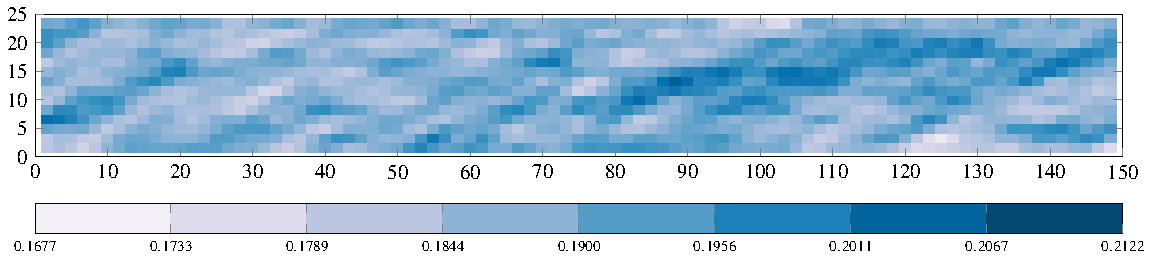
\includegraphics[width=0.9\textwidth]{volfrac_map_md600}}\\
	\subfloat[][$\gamma=1.0$\label{fig:TS_sbens}]{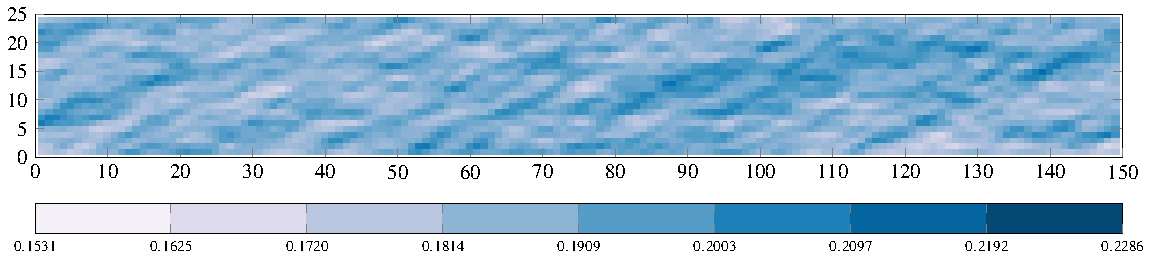
\includegraphics[width=0.9\textwidth]{volfrac_map_md1000}}\\
	\subfloat[][$\gamma=2.0$\label{fig:TS_bsens}]{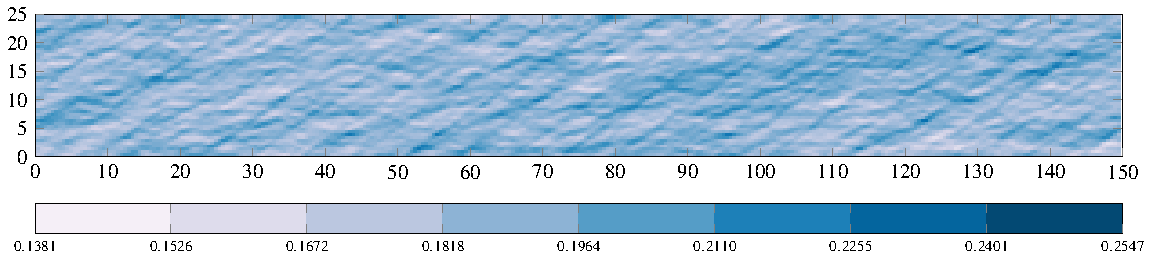
\includegraphics[width=0.9\textwidth]{volfrac_map_md2000}}
	\caption{Refining the volume fraction auxiliary map according to the mesh density for one realisation ($\text{SD}=20$)}
	\label{fig:volfrac_maps}
\end{figure}%
\afterpage{\clearpage}

\begin{figure}[!h]{}
  	\centering
	\subfloat[][$\gamma=0.1$\label{fig:S_sehns}]{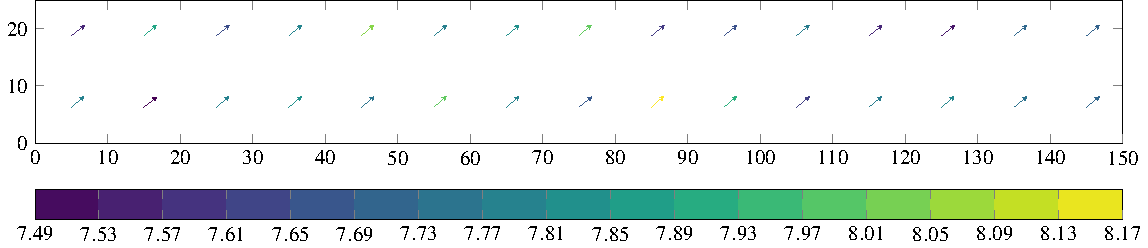
\includegraphics[width=0.9\textwidth]{tensor_map_md100}}\\
	\subfloat[][$\gamma=0.2$\label{fig:S_senfs}]{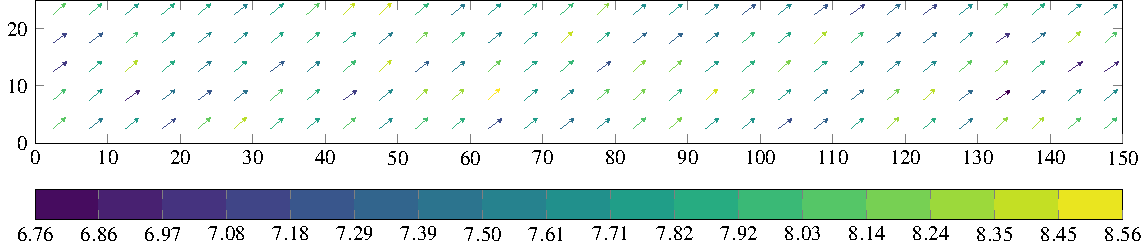
\includegraphics[width=0.9\textwidth]{tensor_map_md200}}\\
	\subfloat[][$\gamma=0.6$\label{fig:S_sens}]{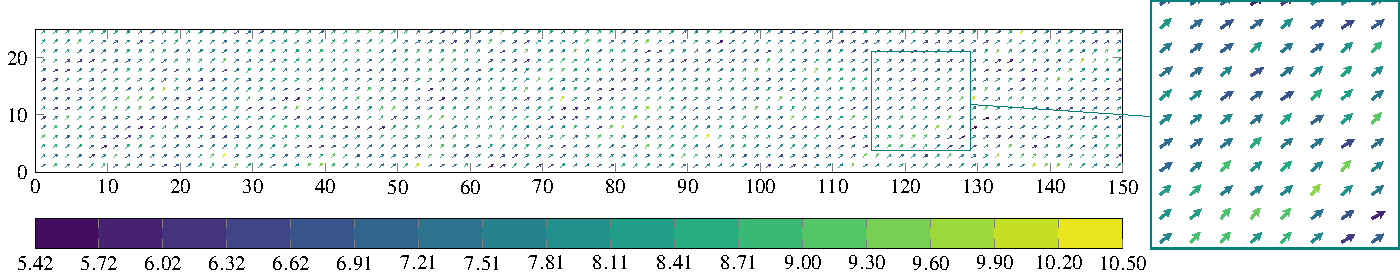
\includegraphics [width=0.9\textwidth] {tensor_map_md600}}\\
	\subfloat[][$\gamma=1.0$\label{fig:S_sbens}]{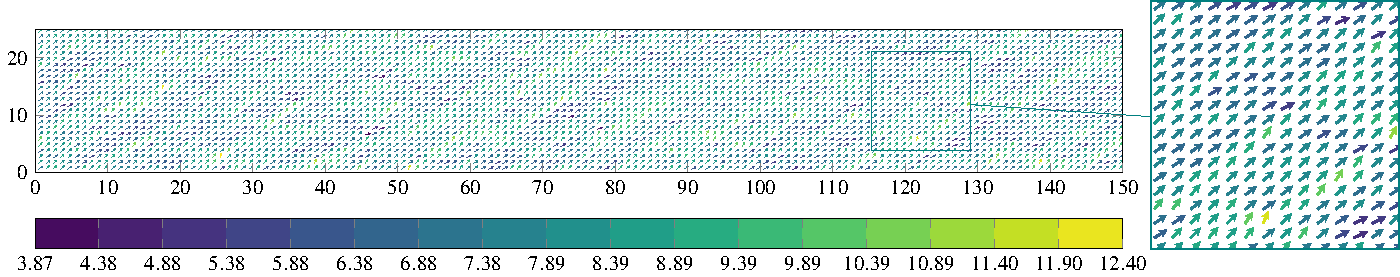
\includegraphics[width=0.9\textwidth]{tensor_map_md1000}}\\
	\subfloat[][$\gamma=1.5$\label{fig:S_bsens}]{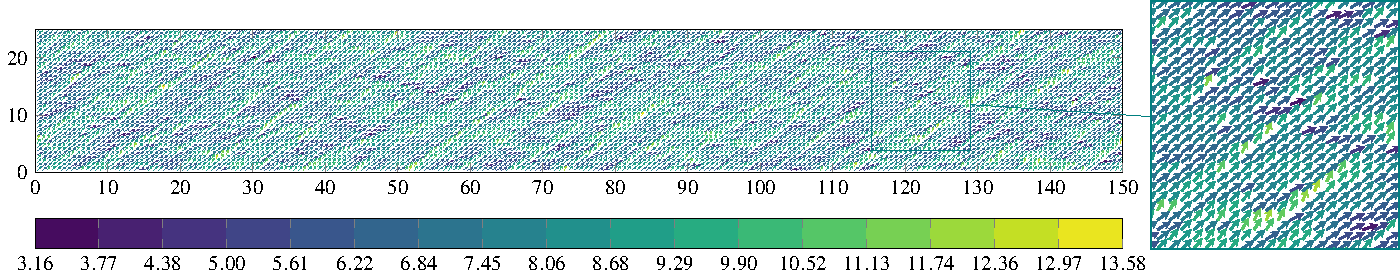
\includegraphics[width=0.9\textwidth]{tensor_map_md1500}}
	\caption{Refining the orientation tensor auxiliary map according to the mesh density for one realisation ($\text{SD}=20$); the principal directions are graphed while the angles are scaled 6 times for clarification}
	\label{fig:tensor_maps}
\end{figure}%


	\paragraph{Parametric study} The parametric study is carried out by varying the SD of the ODF, which is a Gaussian distribution as reported in~\autocite{Virk.2013}. Setting the SD to zero for the orientation distribution results in the special case of aligned fibres along the mean angle of the distribution ($7.36^\circ$). Namely, the global orientation corresponds to the local one for each element. Therefore, the first point in Fig.~\ref{fig:mesh_param} represents the global calculation that results in a mean Young's modulus of 8965.86\,MPa. Similarly, the following five points, all below $\text{SD}=5$, result in values close to the initial perfectly aligned case. The obtained results from the local analysis do not show a significant difference compared to the global value. A rather sharp drop in stiffness is observed for values over SD of 5. Moreover, the results seems to be more spread out for higher values. Interestingly, the experimental value was recorded for the SD of 17.95, which is best estimated by the local FE realisations in the range of 15--17.5. Note that the experimental value is quite distant with respect to the global value and even the local values with low SD. More specifically in Table~\ref{table:results7}, global and low-variation local Young's moduli results show relative errors of around 9\% whereas the local analysis of $\text{SD}=17.95$ contains half as much error. One could argue that based on the local FE results, the estimation of the ODF in~\autocite{Virk.2013} by the SDs in the range of 15--17.95 seems to be plausible.


\begin{figure}[!h]{}
  	\centering
  	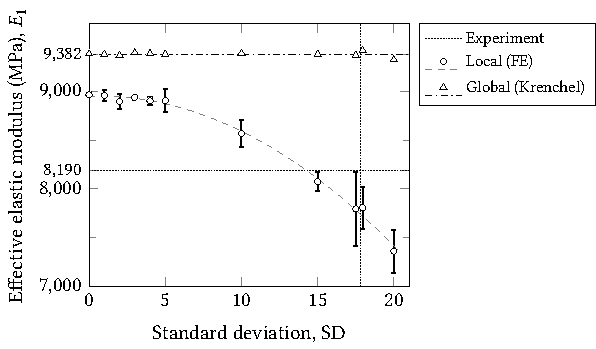
\includegraphics[scale=1]{E_parametric}
	\caption{Parametric result of all realisations along with SD error bars; the experimental value of 8190 was reported for $\text{SD}=17.95$ in~\autocite{Virk.2013}}
	\label{fig:mesh_param}
\end{figure}%
	
	As a measure of global behaviour, Krenchel's formulation is used assuming that all the fibres are oriented along the mean angle, see Table~\ref{table:results7}. The angle is obtained from the eigenvector of the principal direction, which is the denoted by the maximum eigenvalue. The behaviour of this analytical model, along with the angle obtained from the FE analysis clearly shows that global behaviour is insensitive to local fibre orientation. This global value overestimates the experimental value by approximately 15\%.
	
	From the micromechanical point of view, focusing on local computation has a secondary benefit: the ergodicity hypothesis remains valid for each element. Thus, what is practically done is introducing an RVE for each element rather than the whole structure. Inexpensive computational cost makes this approach practical. This assumption allowed to remove an element when the scale separation hypothesis collapses due to failure---without affecting other elements.	


\begin{table}[!hb]
\centering\scriptsize
\caption{Experimental and numerical results for the effective elastic modulus of the composite ($E_1$, in MPa), and relative error in percentage}\label{table:results7}
\begin{tabular}{l@{\hspace{0.1cm}}l@{}*{11}{c}}
\toprule
\multicolumn{2}{l}{\multirow{2}{*}{\bfs{Composite property}}}  &  \multicolumn{11}{c}{\bfs{Standard deviation of angle distribution}} \\                                                           
\cmidrule(l{0cm}r{0cm}){3-13} && \hfil\bfs{0}&\hfil\bfs{1}&\hfil\bfs{2}&\hfil\bfs{3}&\hfil\bfs{4}&\hfil\bfs{5}&\hfil\bfs{10}&\hfil\bfs{15}&\hfil\bfs{17.5}&\hfil\bfs{17.95}& \hfil\bfs{20}\\	
\toprule
%\multirow{3}{*}{$E_\text{Local}$}& Mean (MPa)			&8965.86	&8958.61 &8897.15	&8940.65 &8903.21 &8905.26&8567.98 &8074.07	&7795.04 &7805.69 &7403.08\\
% The previous line was change to the following to keep the same number of significant digits for both values and their SDs.
\multirow{3}{*}{$E_\text{Local}$}& Mean (MPa)			&8966	&8959 &8897	&8941 &8903 &8905&8568 &8074&7795 &7806 &7403\\
%					&SD (MPa)				&23.33	&53.76   &74.20	    &26.65	 &42.32	  &120.40 &	135.48 &98.19	&381.70	 & 215.77 &264.99\\
					&SD (MPa)				&23.33	&53.76   &74.20	    &26.65	 &42.32	  &120.4 &	135.5 &98.19	&381.7	 & 215.8 &264.9\\
&Relative error (\%) &9.47    &9.38      &8.63	 &9.17	  &8.71   &8.73	   &4.62	&1.42	 &4.82	  &4.69	&10.13\\\midrule
\multirow{2}{*}{$\theta_\text{Global}$}&Mean   &7.36&7.41&7.59&7.17&7.29&7.41&7.27&7.39&7.56&6.79&8.23\\
&SD&0.00&0.25&0.40&0.13&0.24&0.17&0.97&0.42&1.81&1.56&1.41\\\midrule
%\multirow{2}{*}{$E_\text{Global}$}&Krenchel (MPa) & 9386.08&	9382.99&9370.84& 9398.16&9390.46&9382.87 &9392.08 &9383.88 &9372.93&9421.69 &9325.91\\
\multirow{2}{*}{$E_\text{Global}$}&Krenchel (MPa) & 9386.08&	9383&9371& 9398&9391&9383 &9392 &9384 &9373&9422 &9326\\
&Relative error (\%)  &14.60&14.57&14.42&14.75&14.66&14.56&14.68&14.58&14.44&15.04&13.87\\
 \bottomrule
\end{tabular}
\end{table}
	
	Obviously, the discussion is based on the few number of realisations. More accurate results could be obtained by increasing the number of realisations to better approximate the ensemble value. Namely, more realisations may decrease the variation of the output but it would not violate the overall observed behaviour.
	


\section{Conclusion}	
	The focus of this work was on developing a simple element-wise semi-numerical scheme to homogenise aligned NFRCs through a cost-effective approach. To this end, after reviewing the concept of orientation tensor and presenting the pertaining constitutive equation, the following points were motivated to consider auxiliary maps:
%	with the potential to be incorporated  multi-scale simulations.
	\begin{itemize}
		\item Local anisotropy (more specifically transverse isotropy for the case of long fibres) and its global counterpart were distinguished from each other. In the former, the elastic stiffness acquires a point-wise transverse symmetry for which the axis of symmetry is a function of location whereas in the latter insensitivity to the local variation is evident.
		\item Accepting the ergodic hypothesis for a material requires statistical homogeneity of its micro-structure (even when random heterogeneities are present). Fulfilling such a condition for the whole structure is quite strong but demanding it element-wisely relaxes the requirements.
	\end{itemize}
	The effective elastic modulus of NFRCs of an experimental study was predicted. Mesh dependency of the results was quickly removed by refining the elements while the auxiliary maps were scaled down to the same extent. It was observed that increasing the SD of ODF over values of 5 highly reduces the effective stiffness of the sample. While lower values of SD overestimated the experimental result, higher values (around the reported SD of the ODF) give plausible estimates within 5\% error range in average. Analytical approach that considers the global average orientation, remained insensitive to local variation.
		
	Based on the obtained results, the following points are suggested:
	\begin{itemize}
		\item Instead of the more common global or layer-wise calculation of the orientation tensor, an element-wise approach should be adopted (where possible). The proposed procedure is in accordance with subdividing the whole structure to finite elements as auxiliary maps followed the same refinement. In addition, auxiliary maps of volume fraction and orientation tensor enabled setting up an independent RVE for each element. 
		\item It was shown that mesh-independent results were obtained using auxiliary maps and through a 2D simple analysis. Namely, projecting all layers onto a single 2D layer does not include much loss of information in regard to orientation. This could be a good recommendation that as a result of specific manufacturing techniques, 3D computation is bypassed. 
	\end{itemize}
	By implementing the suggestions of the current study, adequate local morphological information was captured and a more accurate, yet computationally inexpensive, simulation of mechanical response was carried out.	

	\paragraph{Future work} Auxiliary map(s) of clustering index and/or damage might be used in conjunction with the introduced maps of the current study to elaborate the understanding of  material response in future works. A comparison between the local and global failure criteria should be carried out to challenge the proposed method in strength calculations---specially when element removal is involved.

